\documentclass[11pt]{article}
\usepackage{graphicx}
\graphicspath{{/Users/justindoty/Documents/Research/Dissertation/Production_QR_Proxy/Code/}}
\usepackage{graphics}
\usepackage{amsfonts}
\usepackage{amsmath}
\usepackage{amstext}
\usepackage{tabularx}
\usepackage{mathrsfs}
\usepackage{subfigure}
\usepackage[dvipsnames]{xcolor}
\usepackage{lscape}
\usepackage{longtable}
\usepackage{bm}
\usepackage{bbm}
\usepackage{chngcntr}
\usepackage{setspace}
\usepackage{caption}
\usepackage{float}
\usepackage{multirow}
\usepackage{booktabs}
\usepackage{natbib}
\usepackage{fancyvrb}
\usepackage{enumitem}
\usepackage[multiple]{footmisc}
\newtheorem{assump}{Assumption}[section]
\newtheorem{lemma}{Lemma}[section]
\newtheorem{theorem}{Theorem}[section]
\newcommand{\indep}{\perp \!\!\! \perp}


\usepackage[multiple]{footmisc}

%Set margins and text size
\setlength{\textwidth}{6.5in} \setlength{\textheight}{8.8in}
\setlength{\topmargin}{-0.5in}
\setlength{\oddsidemargin}{-0.01in}{}
\setlength{\parskip}{1.6mm}
\parskip=.06in
{}
%Some useful short-cuts
\def\argmax{\mathop{\rm arg\,max}}
\def\argmin{\mathop{\rm arg\,min}}



\setcounter{section}{0} % starts numbering section 1start_value=[0.498,-0.2874,0.4314,0.5444];

\setcounter{page}{1}



\usepackage{hyperref}
\hypersetup{
    colorlinks=true,
    allcolors=Violet
}
\begin{document}

\title{Heterogeneity in Firms: \\
A Proxy Variable Approach for Quantile Production Functions
%\footnote{}
}

\author{Justin Doty\thanks{Department of Economics, University of Iowa, S321 Pappajohn Business Building, 21 E Market St, Iowa City, IA 52242. Email: \href{mailto:justin-doty@uiowa.edu}{\texttt{justin-doty@uiowa.edu}}} and Suyong Song\thanks{Department of Economics and Finance, University of Iowa, W360 Pappajohn Business Building, 21 E Market St, Iowa City, IA 52242. Email: \href{mailto:suyong-song@uiowa.edu}{\texttt{suyong-song@uiowa.edu}}}
}

\date {\today}
\maketitle


\begin{abstract}
We propose a new approach to estimate production functions in which output elasticities are heterogeneous across the firm size distribution. 
This paper extends the proxy variable approach for estimating production functions to the conditional quantiles of firm production. Production function parameters are estimated in a simple two-stage approach which relies a location-shift assumption on unobserved productivity. We show that this method allows us to capture heterogeneity in output elasticities along the firm size distribution that may not be found in conditional mean estimates of \cite{Levinsohn2003} and \cite{Ackerberg2015}. We provide small-sample evidence in a Monte Carlo study to show that this approach is robust compared to other production function estimators. The method is applied to plant-level manufacturing data from Chile and Colombia.
\end{abstract}


\textit{Keywords:} Production functions, Heterogeneous elasticity, Quantile regression

\textit{JEL Classification:} C14, C36, D24


\pagenumbering{arabic}

\baselineskip25pt

%\singlespacing
\onehalfspacing
%\doublespacing

\section{Introduction}

Production function estimation is an ongoing and historical empirical research topic that links firm's input to output decisions. Identification of the output elasticities and consequently the distribution of firm-level productivity is constrained by endogeneity issues. This is because productivity is unobserved by the econometrician, but observed by the firm when making input decisions. 

A popular approach to address this issue is to introduce a proxy variable such as investment, made popular by \cite{Olley1996} (OP) or an intermediate input using \cite{Levinsohn2003} (LP) or \cite{Ackerberg2015} (ACF). These proxies are functions of a state variable such as capital and unobserved productivity. Under certain assumptions, this function is strictly increasing in its scalar unobserved productivity component. Inverting this function controls for unobserved productivity and the production function parameters can be estimated with a simple two-stage estimator.

While these methods have been useful in identifying the production function parameters and recovering consistent estimates of total factor productivity (TFP), resulting estimates may be biased if there is additional heterogeneity in production technology across firms. Thus, allowing for heterogeneous coefficients is one possible way to capture these differences. The literature on heterogeneous production functions is small relative to the empirical research using the homogeneous coefficient model, even though many empirical studies have found heterogeneity in firm behavior and decisions.\footnote{Some notable examples are \cite*{Kasahara2015}, \cite*{balat} and \cite*{Li2017} to name of few. Also \cite{Gandhi2020} who estimate a nonparametric production function and obtain heterogeneous estimates.} This is because estimating the homogeneous coefficient model by itself is very difficult due to the issue of unobserved productivity. 

In our approach, we allow for non-neutrality of the unobserved idiosyncratic production shock, but require the component of productivity that is anticipated by firms to be Hicks-neutral.  We use the proxy variable approach in this framework in order to control for the part of production unobservables that are correlated with input decisions. The literature on control function approaches for quantile regression models is still a developing area therefore it is not straightforward to estimate production functions by allowing for endogenous inputs and their heterogeneous coefficients.\footnote{See for example \cite{Chesher2003}, \cite{Ma2006}, \cite{Lee2007} and \cite{2009a}} We are not aware of any published paper which takes into account the endogeneity issue of production functions in the conventional quantile regression framework. We fill the gap in this paper by proposing an easy-to-implement estimator.

We show through simulation, that our proposed two-step estimator performs well when productivity is estimated using the static control function approaches of either \cite{Levinsohn2003} or \cite{Ackerberg2015}. The estimator is successful in capturing  both heterogeneous output elasticities and controlling for unobserved productivity. In our empirical application, we consider several popular firm and plant-level manufacturing datasets and compare our estimator to the ACF estimator. We show that heterogeneity in these estimates implies differences in other features of firm production, such as returns to scale, capital intensity and productivity.

The rest of the paper is organized as follows. Section \ref{litreview} reviews prior approaches for production function estimation and the interpretations of quantile production functions. Section \ref{ourmodel} introduces the econometric model and the proposed estimator. Section \ref{montecarlo} presents finite-sample behaviors of the estimator via Monte Carlo experiments and Section \ref{application} applies this estimator to US, Chilean, and Colombian manufacturing datasets. Section \ref{conclusion} concludes with directions for future research.

\section{Literature Review} \label{litreview}
\subsection{Production Function Estimation}

We briefly review the ACF (2015) procedure for estimating a \textit{value-added} production function (in logs):

\begin{equation}
y_{it}=\beta_{k}k_{it}+\beta_{l}l_{it}+\omega_{it}+\eta_{it},
\end{equation}
where $y_{it}$ denotes value-added output for firm $i$ at time $t$, $l_{it}$ denotes labor input, $k_{it}$ denotes capital input, $\omega_{it}$ is unobserved productivity and $\eta_{it}$ denotes an iid shock to production.\footnote{We omit the constant $\beta_{0}$ because it is not separately identified from the mean of productivity}

To control for the correlation between $\omega_{it}$ and inputs $k_{it}$ and $l_{it}$, ACF introduces an intermediate input demand defined as
\begin{equation}
m_{it}=m_{t}(k_{it}, l_{it}, \omega_{it}),
\end{equation}
where the function $m$ is strictly increasing in $\omega_{it}$ for all $k_{it}$ and $l_{it}$. Productivity can then be expressed as
\begin{equation}
\omega_{it}=m_{t}^{-1}(k_{it}, l_{it}, m_{it}).
\end{equation}
Substituting this equation into the production function they obtain
\begin{equation}
y_{it}=\beta_{0}+\beta_{k}k_{it}+\beta_{l}l_{it}+m^{-1}_{t}(k_{it}, l_{it}, m_{it})+\eta_{it}=\Phi(k_{it}, l_{it}, m_{it})+\eta_{it}.
\end{equation}
The function, $\Phi_{t}(k_{it}, l_{it}, m_{it})$, is identified by the following first stage moment restriction
\begin{equation}
\mathbb{E}[\eta_{it}|\mathcal{I}_{it}]=\mathbb{E}[y_{it}-\Phi_{t}(k_{it}, l_{it}, m_{it})|\mathcal{I}_{it}]=0,
\end{equation}
where $\mathcal{I}_{it}$ denotes the firm's information at time $t$. The first stage estimate of $\Phi_{t}$ can be obtained by a local linear regression or a polynomial regression in $(k_{it}, l_{it}, m_{it})$. This step controls for the unobservable $\eta_{it}$.

A second stage moment restriction identifies the coefficient on capital and labor. Assume that productivity follows an auto-regressive process
\begin{equation}
\omega_{it}=\mathbb{E}[\omega_{it}|\omega_{it-1}]+\xi_{it}=g(\omega_{it-1})+\xi_{it}
\end{equation}
where $\xi_{it}$ denotes an innovation to productivity and satisfies $\mathbb{E}[\xi_{it}|\mathcal{I}_{it-1}]=0$.

Then, the production function parameters can be estimated from the moment restrictions corresponding to orthogonality assumptions on the productivity innovation, $\xi_{it}$ by expressing productivity as a function of the parameters $\beta_{k}$ and $\beta_{l}$
\begin{equation}
\mathbbm{E}\Bigg[\hat{\xi}_{it}(\beta_{k}, \beta_{l})\otimes
\begin{pmatrix}
k_{it}\\
l_{it-1}
\end{pmatrix}\Bigg]=0
\end{equation}
where $\hat{\xi}_{it}(\beta_{k}, \beta_{l})$ is constructed from the residuals of a regression of $(\widehat{\beta_{0}+\omega_{it}})=\hat{\Phi}_{t}(k_{it}, l_{it}, m_{it})-\beta_{k}k_{it}-\beta_{l}l_{it}$ on its lagged value for a hypothetical value of $(\beta_{k}, \beta_{l})$.  

\subsection{Production Functions and Quantile Regression}


A quantile regression framework for production functions may facilitate many different interpretations. Since this framework has been applied in the production frontier literature, we briefly review how this may be a natural interpretation and the limitations of such a model. A (stochastic) frontier (SFA) model of production proposed by \cite{Aigner1977} introduces statistical error into a frontier model. Frontier models assume firms firms deviate from an optimal frontier of production. The SFA model is typically written as
\begin{equation}
y_{i}=f(x_{i}, \beta)+\varepsilon_{i},
\end{equation}
where $\varepsilon_{i}=\eta_{i}-u_{i}$, $x_{i}$ are inputs to production and $\beta$ are the parameters. The error term $\eta_{i}$ denotes the statistical noise in the model such as measurement error and $u_{it}$ represents one-sided deviations from the production frontier. Estimates of $\beta$ are typically obtained using maximum likelihood which requires strong distributional assumptions on the error terms. \cite{Bernini2004} suggests quantile regression could be used to estimate the highest percentiles of the conditional output distribution as an estimate of the production frontier. \cite{Aragon2005} uses a characterization of a deterministic frontier that interprets production functions as being from a continuous interval $\tau\in[0,1]$ where $\tau=1$ corresponds to the efficient frontier. The difficulty with these approaches is choosing which quantile to estimate as the frontier and performing inference on these extremal quantiles.\footnote{See \cite{Chernozhukov2005a} on how to extend inference in quantile regression to extreme tails in the conditional distribution} Predicting differences between the frontier and a production process for a given firm is also complicated since the predicted error is a composite of technical inefficiency and noise. Other econometric issues, such as endogeneity of input choices with respect to inefficiency are difficult to incorporate in this framework. The purpose of this paper is not to debate the advantages and disadvantages of production frontier models so we leave this discussion for future studies and acknowledge the theoretical challenges of quantile frontiers and instead focus on the standard production function model.

There are two main challenges with implementing a quantile regression framework to the standard production function model. First, addressing the endogeneity of $\omega_{it}$ using traditional panel data methods or control function approaches for quantile models is still a developing field that faces many challenges such as incidental parameters or non-smooth criterion functions. Second, it is not straightforward to link firms output decisions to variations in the ex-post shock $\eta_{it}$ without imposing some strict structural model of firm production.

Addressing the first point, we will argue that recent quantile panel data and quantile IV models should not be used for the same reasons panel data and IV models are not used for the conditional mean model. Quantile panel data models allow for flexible interactions between unobserved heterogeneity and the quantiles of the conditional response function. Some well known approaches assume a time-invariant fixed effect such as \cite{Koenker2004}, \cite{Lamarche2010}, or \cite{Canay2011} which assumes the fixed effect shifts only the location of the conditional quantile function. This approach has two disadvantages. First, assuming the unobservable is time-invariant is restrictive. \cite{Griliches1986} show that a fixed effect for productivity, $\omega_{i}$, leads to low estimates of the capital elasticity. Second, with the exception of the \cite{Canay2011} estimator, the fixed effects of these models are incidental parameters so as the sample size grows, so does the number of parameters that need to be estimated which makes it computationally costly. An alternative to fixed effect estimation is to model the unobserved heterogeneity as a projection onto the observables plus a disturbance in the spirit of \cite{Chamberlain1984}. This correlated random effect (CRE) approach was used by \cite{Abrevaya2008} and variations of this type of estimator have been developed by other researchers. One issue with the CRE approach is that identification of the conditional quantile function is difficult because it now depends on the joint distribution of unobservables in the response function and the random effect.

Another alternative is to make use of valid instruments if they are available. The conventional argument for using input prices $p^{k}_{it}$ and $p^{l}_{it}$ as instruments is that they must be uncorrelated with the error term $\omega_{it}+\eta_{it}$ and correlated with input choices for capital and labor. Then one could use two-stage least squares to obtain consistent estimates of $\beta_{k}$ and $\beta_{l}$. This idea can be extended to quantile-IV models such as \cite{Chernozhukov2005}. In their identification arguments, one would need to strengthen assumptions to conditional independence as well as monotonicity of a quantile structural function (QSF) in $U_{it}=\omega_{it}+\eta_{it}$. Then if one writes the QSF for the production function as $y_{it}=Q(k_{it}, l_{it}, U_{it})$, their the model is identified using
\begin{equation}
P[y_{it}\leq Q_{\tau}(y_{it}|k_{it}, l_{it})|k_{it}, l_{it}, p^{k}_{it}, p^{l}_{it}]=\tau, \quad \tau\in (0,1].
\end{equation}
We do not use this procedure since input prices may not have enough variation across firms and exogeneity can be violated if they capture input quality differences as shown by \cite{Griliches1986}. Therefore, it is not straightforward to develop an identification strategy that also leads to a computationally simple estimator. This is a common challenge in the quantile IV literature. However, we will show that a simple adaption of the \cite{Canay2011} estimator works well in practice.


\section{A Random Coefficient Production Function} \label{ourmodel}
We specify a \textit{value-added} production function as a random coefficient model:
\begin{equation} \label{pfrc}
    y_{it}=\beta_{k}(\eta_{it})k_{it}+\beta_{l}(\eta_{it})l_{it}+\omega_{it}
\end{equation}
The variables in equation \eqref{pfrc} have the same interpretation as the ones we introduced in the ACF model. In this specification we allow the output elasticities to be functionally dependent on the production shock $\eta_{it}$ while productivity $\omega_{it}$ maintains its additive separability. The model presented here assumes that $\omega_{it}$ is only a location-shift of the conditional output distribution. We assume the constant in the production function does not vary over $\tau$ since the constant is not separately identified from the mean of productivity. The location-shift specification is crucial in our approach since $(\beta_{0}+\omega_{it})$ also appears in the conditional mean counterpart of equation \eqref{pfrc} so that if this object can be consistently estimated from popular proxy variable approaches such as OP, LP or ACF, then with additional restrictions from the quantile IV literature, the production function parameters $\beta_{k}(\tau)$ and $\beta_{l}(\tau)$ can also be consistently estimated.

We should also mention that a value-added specification in equation \eqref{pfrc} is non-trivial. Value-added production functions are common in the empirical literature, however the objects recovered from a value-added model such as the output elasticities and TFP can only be mapped to its gross-output counterpart under special structural production functions such as Leontief value-added. Since the production shock $\eta_{it}$ enters \eqref{pfrc} non-separably, it is difficult to recover gross-output objects from value-added since the latter is composed of the additional error term. One consequence of a value-added model is that estimates of productivity may be more disperse than gross-output estimates which controls for material inputs. Therefore, in our empirical application we interpret the elasticities and productivity with some caution.

 One advantage of the value-added model is that the rank of $\eta_{it}$ can be interpreted as the rank of firm size measured by output net of material inputs. This way, we are able to measure firm size by the value of the firm's contribution to output rather than the value of the units they sell. The value-added approach also avoids the non-identification results of \cite{Gandhi2020}. We leave the connection between this value-added production function and its possibly underlying gross-output production function as future research agenda.

 An interesting question that follows from the firm size interpretation is then what are the determinants of firm size? Controlling for productivity also controls for firm size determinants such as managerial ability so variation in firm size might be limited in our model. There is a large and historical literature on the determinants of firm size. \cite{Kumar1999} survey some of the theories and test them using data. We offer a possible explanation below, but we focus on whether there is heterogeneity in firm size and its consequences. 

A special case of \eqref{pfrc} is the location-scale model,

\begin{equation} \label{locationscale}
    y_{it}=\beta_{k}k_{it}+\beta_{l}l_{it}+\omega_{it}+(\mu_{k}k_{it}+\mu_{l}l_{it})\eta_{it}
\end{equation}
Which implies that the $\tau$-th conditional quantile of $y_{it}$ is given by

\begin{equation}
Q_{\tau}(y_{it}|\mathcal{I}_{it})=\beta_{k}k_{it}+\beta_{l}l_{it}+\omega_{it}+(\mu_{k}k_{it}+\mu_{l}l_{it})F^{-1}(\tau)
\end{equation}
where $F^{-1}(\tau)$ is the quantile function of production shocks $\eta_{it}$.

The idea that input choices can impact firm's production beyond the conditional mean has important consequences for firm's attitude towards production risk. A volume of literature that originated in the late 1970's challenged the standard stochastic specifications of production functions \citep{Just1978,Just1979} by considering a specification that allowed firm's inputs to both increase or decrease the marginal variability of final output. These models are commonly applied to studying the agricultural industry where the variance on the yield of harvested crops could be increased by adverse weather or decreased by pesticide usage. Since manufacturing businesses tend to operate in a more controlled environment, risk is less prevalent in these industries so the conditional variance of $\eta_{it}$ may be smaller.

The connection between production risk and heterogeneity in quantiles is interesting so we briefly mention that under quantile preferences, a firm who maximizes the $\tau$ level of utility of profits could explain heterogeneity in the output distribution. Unlike risk-neutral firms, firms could have a utility function that is represented by preferences of the firm manager(s) who decides the optimal expenditure on inputs. Different managers may have different preferences for risk. A short list of papers have considered quantile utility maximization such as \cite{Manski1988}, \cite{ROSTEK2009}, \cite{Chambers2007}, and \cite{Bhattacharya2009}. Dynamic input choices such as investment are much more difficult to solve using the quantile utility framework and the reader can refer to \cite{Castro2017} for a treatment of dynamic quantile utility models. As far as we know, the quantile utility framework has not been applied to firm decision problems and a more thorough treatment of such is outside the scope of this paper.

A general quantile model such as the one specified in \eqref{pfrc} can be seen as an extension of the higher-order moment estimation of risk initiated by \cite{Antle1983}. However, it can also be seen purely as an econometric specification issue as we are unaware of any tests that could distinguish between higher order moment production risk and misspecification. We choose the latter interpretation for our model. 

\subsection{Identification}

We show that the production function coefficients $\boldsymbol{\beta}(\tau)=(\beta_{k}(\tau), \beta_{l}(\tau))$ are non-parametrically identified with $T=2$ under conditional independence assumptions and other mild regularity conditions used in conditional deconvolution arguments. Similar ideas have been used in panel data models such as \cite{Canay2011}, \cite{Neumann2007}, and \cite{evdo2010}. To simplify notation, we let $x_{i1}=(k_{i1}, l_{i1}), x_{i2}=(k_{i2}, l_{i2})$ and $x_{i}=(x_{i1}, x_{i2})$. Let $Z_{it}=\beta_{k}(\eta_{it})k_{it}+\beta_{l}(\eta_{ti})l_{it}$ for $t\in\{1,2\}$. We then write two consecutive period of output as $y_{i1}&=Z_{i1}+\omega_{i1}$ and $y_{i2}&=Z_{i2}+\omega_{i2}$. We assume a linear AR(1) process for productivity $\omega_{i2}=\rho\omega_{i1}+\xi_{i2}$. Plugging into the second line of the previous equation allows us to write $y_{i2}=Z_{i2}+\rho\omega_{i1}+\xi_{i2}$. Dividing by $\rho$ we write $\tilde{y}_{i2}=y_{i2}/\rho=\tilde{Z}_{i2}+\tilde{\xi}_{i2}+\omega_{i1}$. Therefore, our two repeated measures of productivity are given by:
\begin{equation} \label{repeatedmeas}
\begin{split}
y_{i1}&=Z_{i1}+\omega_{i1}\\
\tilde{y}_{i2}&=\tilde{Z}_{i2}+\tilde{\xi}_{i2}+\omega_{i1}
\end{split}
\end{equation}
 We present our identification argument in two steps. In the first steps, we utilize conditional deconvolution arguments to identify relevant conditional characteristic functions which are known up to parameters $\rho$ as well as the mean production coefficients $\boldsymbol{\beta}^{\mu}=(\beta_{k}^{\mu}, \beta_{l}^{\mu})=\mathbbm{E}[\boldsymbol{\beta}(\eta_{it})]$. In the second step, we argue that these parameters are identified by standard assumptions in the proxy variable approach of \cite{Olley1996}, \cite{Levinsohn2003}, or \cite{Ackerberg2015} which are both based on conditional mean restrictions. We begin with some assumptions.

\begin{assump} \label{idpart1}
Suppose the following set of assumptions 
	\begin{enumerate}[label=(\alph*)]
		\item Random Sample: The random variables $(y_{i}, Z_{i}, \omega_{i})_{i=1}^{N}$ are identically and independently distributed and $T=2$
		\item Conditional Independence: (i) $f_{Z_{it}|x_{i}, Z_{is}, \omega_{it}}(Z_{it}|x_{i}, Z_{is}, \omega_{it})=f_{Z_{it}|x_{i}}(Z_{it}|x_{i})\, \forall t\neq s$ and $t\in\{1,2\}$ and (ii) $f_{\xi_{i2}|x_{i}, Z_{it}, \omega_{i1}}(\xi_{i2}|x_{i}, Z_{it}, \omega_{i1})=f_{\xi_{i2}|x_{i}}(\xi_{i2}|x_{i})$ for $t\in\{1,2\}$
		\item Characteristic Functions: The conditional characteristic functions $\phi_{Z_{i1}|x_{i}}(s|x_{i})$, $\phi_{\omega_{i1}|x_{i}}(s|x_{i})$ and $\phi_{\xi_{i2}|x_{i}}(s|x_{i})$  do not vanish $\forall s\in \mathbbm{R}$
		\item Quantiles: $\eta_{it}\indep (x_{i}, \omega_{it})$ where $\eta_{it}\sim U[0,1]$ and $Z_{it}$ is strictly increasing in $\eta_{it}$
	\end{enumerate}
\end{assump}
In addition to Assumption \ref{idpart1} we restate and augment the assumptions in \cite{Ackerberg2015}
\begin{assump} \label{idpart2}
Suppose the following set of assumptions 
	\begin{enumerate}[label=(\alph*)]
		\item Information Set: The firm's information set at time $t$ is given by $\mathcal{I}_{it}$ and includes current and past productivity shocks, but does not include future productivity shocks
		\item Productivity: The evolution of productivity follows a linear AR(1) process: $\omega_{it}=\rho\omega_{it-1}+\xi_{it}$ where $\mathbbm{E}[\xi_{it}|\mathcal{I}_{it-1}]$ and $\omega_{it}$ is strictly stationary, $f_{\omega_{i1}}(\omega_{i1})=f_{\omega_{i2}}(\omega_{i2})$
		\item Timing of  Input Choices: Firms accumulate capital according to
		\begin{equation*}
		k_{it}=\kappa(k_{it-1}, k_{it-1})
		\end{equation*}
		\item Scalar Unobservable: Firm's intermediate input demand is given by
		\begin{equation*}
		m_{it}=m_{t}(k_{it}. l_{it}, \omega_{it})
		\end{equation*}
		\item Strict Monotonicity: $m_{t}(k_{it}. l_{it}, \omega_{it})$ is strictly increasing in $\omega_{it}$
		\item Location: $\boldsymbol{\beta}^{\mu}=(\beta_{k}^{\mu}, \beta_{l}^{\mu})=\mathbbm{E}[\boldsymbol{\beta}(\eta_{it})]$ is non-singular with finite norm
	\end{enumerate}
\end{assump}

Assumption \ref{idpart1}(b)(i) implies that the ex-post production shocks are mutually independent over time and independent from productivity $\omega_{it}$. This is a potentially strong condition, but commonly used in nonseparable panel data models. Related conditions are used in \cite{Hu2019} who assume that $\eta_{it}$ is independent of $\omega_{it}$ conditional an $x_{i}$. Part (ii) of this assumption implies that the innovation shocks to productivity $\xi_{it}$ are independent of the ex-post shocks $\eta_{it}$ and that these shocks are independent of lagged productivity $\omega_{it-1}$. Assumption \ref{idpart1}(c) are mild technical conditions on characteristic functions. Most standard families of distributions satisfy this property. Lastly, \ref{idpart1} (d) extends the independence assumptions of $\eta_{it}$ and $\omega_{it}$ to $x_{i}$. A similar independence assumption is used in \cite{Gandhi2020}. This assumption is used to identify the relevant conditional quantiles.

Assumption \ref{idpart2} extends some of the assumptions in \cite{Ackerberg2015} to identify $\boldsymbol{\beta}^{\mu}$ and $\rho$ which are necessary in our deconvolution argument. \ref{idpart2}(b) requires productivity to follow an linear AR(1) process. Although restrictive, this allows us to easily adapt a repeated measure type argument used for deconvolution. Strict stationarity is also restrictive and is used to achieve identification of the marginal distribution of productivity for each time period. \ref{idpart2}(f) implies that $\boldsymbol{\beta}^{\mu}$ exists which is also assumed in \cite{Canay2011} so that the location of $Z_{it}$ is well defined. With these assumptions stated we are now ready to state the main identification result.

\begin{theorem}
Under Assumptions \ref{idpart1} and \ref{idpart2}, the location $\boldsymbol{\beta}^{\mu}$, coefficient $\rho$ and function $\boldsymbol{\beta}(\tau)$ are identified
\end{theorem}
\textit{Proof:}
Using Assumption \ref{idpart1}(b)(i) we can write the characteristic functions of \eqref{repeatedmeas} as
\begin{equation} \label{repchar}
\begin{split}
\phi_{y_{i1}|x_{i}}(s|x_{i})&=\phi_{Z_{i1}|x_{i}}(s|x_{i})\phi_{\omega_{i1}|x_{i}}(s|x_{i})\\
\phi_{\tilde{y}_{i2}|x_{i}}(s|x_{i})&=\phi_{\tilde{Z}_{i2}|x_{i}}(s|x_{i})\phi_{\tilde{\xi}_{i2}|x_{i}}(s|x_{i})\phi_{\omega_{i1}|x_{i}}(s|x_{i})\\
\end{split}
\end{equation}
The joint characteristic function of $(y_{i1}, \tilde{y}_{i2})|x_{i}$ can then be written as:
\begin{equation} \label{jointchar}
\begin{split}
\Psi_{&(y_{i1}, \tilde{y}_{i2})|x_{i}}(s_{1}, s_{2}|x_{i})=\mathbbm{E}[\exp(i[s_{1}y_{i1}+s_{2}\tilde{y}_{i2}])|x_{i}]\\
&=\mathbbm{E}[\exp(i[s_{1}Z_{i1}+s_{2}\tilde{Z}_{i2}+s_{2}\tilde{\xi}_{i2}+(s_{1}+s_{2})\omega_{i1}])|x_{i}]\\
&=\phi_{Z_{i1}|x_{i}}(s_{1}|x_{i})\phi_{\tilde{Z}_{i2}|x_{i}}(s_{1}|x_{i})\phi_{\tilde{\xi}_{i2}|x_{i}}(s_{1}|x_{i})\phi_{\omega_{i1}|x_{i}}((s_{1}+s_{2})|x_{i})
\end{split}
\end{equation}
where the last equality of \eqref{jointchar} uses Assumption \ref{idpart1}(b)(i-ii). Taking the derivative of \eqref{jointchar} with respect to its first component yields
\begin{equation*}
\begin{split}
\partial_{s_{1}}\Psi_{(y_{i1}, \tilde{y}_{i2})|x_{i}}(s_{1}, s_{2}|x_{i})&=\partial_{s_{1}}\phi_{Z_{i1}|x_{i}}(s_{1}|x_{i})\phi_{\tilde{Z}_{i2}|x_{i}}(s_{1}|x_{i})\phi_{\tilde{\xi}_{i2}|x_{i}}(s_{1}|x_{i})\phi_{\omega_{i1}|x_{i}}((s_{1}+s_{2})|x_{i})\\
&+\phi_{Z_{i1}|x_{i}}(s_{1}|x_{i})\phi_{\tilde{Z}_{i2}|x_{i}}(s_{1}|x_{i})\phi_{\tilde{\xi}_{i2}|x_{i}}(s_{1}|x_{i})\partial_{s_{1}}\phi_{\omega_{i1}|x_{i}}(s_{1}+s_{2}|x_{i})
\end{split}
\end{equation*}
Thus,
\begin{equation*}
\frac{\partial_{s_{1}}\Psi_{(y_{i1}, \tilde{y}_{i2})|x_{i}}(s_, -s|x_{i})}{\Psi_{(y_{i1}, \tilde{y}_{i2})|x_{i}}(s, -s|x_{i})}=\frac{\phi^{'}_{Z_{i1}|x_{i}}(s|x_{i})}{\phi_{Z_{i1}|x_{i}}(s|x_{i})}+\frac{\phi^{'}_{\omega_{i1}|x_{i}}(0|x_{i})}{\phi_{\omega_{i1}|x_{i}}(0|x_{i})}
\end{equation*}
where $\phi_{\omega_{i1}|x_{i}}(0|x_{i})=1$ and $\phi^{'}_{\omega_{i1}|x_{i}}(0|x_{i})=i\mathbmm{E}[\omega_{i1}|x_{i}]$ by properties of characteristic functions. We first discuss identification of $\mathbmm{E}[\omega_{i1}|x_{i}]$. Note that,
\begin{equation*}
\begin{split}
\mathbmm{E}[\omega_{i1}|x_{i}]&=\mathbbm{E}[y_{i1}-Z_{i1}|x_{i}]=\mathbbm{E}[y_{i1}-x_{i1}\beta(\eta_{i1})|x_{i}]=\mathbbm{E}[y_{i1}|x_{i}]-x_{i1}\mathbbm{E}[\beta(\eta_{i1})|x_{i}]\\
&=\mathbbm{E}[y_{i1}|x_{i}]-x_{i1}\mathbbm{E}[\beta(\eta_{i1})]=\mathbbm{E}[y_{i1}|x_{i}]-x_{i1}\boldsymbol{\beta}^{\mu}
\end{split}
\end{equation*}
where the second to last equality follows from the independence assumption in \eqref{idpart1}(d). In order to identify $\mathbmm{E}[\omega_{i1}|x_{i}]$ we must identify $\boldsymbol{\beta}^{\mu}$. The location parameters are identified by Assumption \ref{idpart2}. Then the conditional characteristic function $\phi_{Z_{i1}|x_{i}}(s|x_{i})$ is identified through
\begin{equation*}
\phi_{Z_{i1}|x_{i}}(s|x_{i})=\exp\Bigg(\int_{0}^{s}\frac{i\mathbbm{E}[y_{i1}\exp(i\gamma(y_{i1}-\tilde{y}_{i2}))|x_{i}]}{\phi_{y_{i1}-\tilde{y}_{i2}|x_{i}}(\gamma|x_{i})}d\gamma-is\mathbmm{E}[\omega_{i1}|x_{i}]\Bigg)
\end{equation*}
Then the characteristic function $\phi_{\omega_{i1}|x_{i}}(s|x_{i})$ is identified using
\begin{equation*}
\phi_{\omega_{i1}|x_{i}}(s|x_{i})=\frac{\phi_{y_{i1}|x_{i}}(s|x_{i})}{\phi_{Z_{i1}|x_{i}}(s|x_{i})}
\end{equation*}
From the productivity process, we have $\tilde{\omega_{i1}}=\omega_{i2}/\rho=\omega_{i1}+\tilde{\xi}_{i2}$. Using Assumption \ref{idpart1}(b)(ii) we can write the characteristic function of $\phi_{\omega_{i2}|x_{i}}(s|x_{i})$ as
\begin{equation*}
\phi_{\tilde{\omega}_{i2}|x_{i}}(s|x_{i})=\phi_{\omega_{i1}|x_{i}}(s|x_{i})\phi_{\tilde{\xi}_{i2}|x_{i}}(s|x_{i})
\end{equation*}
Then using Assumption \ref{idpart2}(b) the characteristic functions $\phi_{\omega_{i1}|x_{i}}(s|x_{i})=\phi_{\omega_{i2}|x_{i}}(s|x_{i})$ so we can write
\begin{equation*}
\phi_{\xi_{i2}|x_{i}}(s|x_{i})=\frac{\phi_{\omega_{i1}|x_{i}}(s|x_{i})}{\phi_{\omega_{i1}|x_{i}}(\rho s|x_{i})}
\end{equation*}
Finally, $\phi_{Z_{i2}|x_{i}}(s|x_{i})$ is identified using
\begin{equation*}
\phi_{Z_{i2}|x_{i}}(s|x_{i})=\frac{\phi_{y_{i2}|x_{i}}(s|x_{i})}{\phi_{\xi_{i2}|x_{i}}(s|x_{i})\phi_{\omega_{i1}|x_{i}}(\rho s|x_{i})}
\end{equation*}
The characteristic functions are identified up to an unknown parameter $\rho$. This parameter is identified from Assumption \ref{idpart2}(b) via the moment condition $\mathbbm{E}[\xi_{it}|\mathcal{I}_{it-1}]=\mathbbm{E}[\omega_{it}-\rho\omega_{it-1}|\mathcal{I}_{it-1}]$ where $\omega_{it}=\hat{\Phi}_{t}(k_{it}, l_{it}, m_{it})-\beta^{\mu}_{k}k_{it}-\beta^{\mu}_{l}l_{it}$ using ACF. Identification of the conditional characteristic function implies identification of the conditional distributions. For example, the distribution of $Z_{i1}|x_{i}$ and $Z_{i2}|x_{i}$ can be recovered using the result of \cite{gil}
\begin{equation*}
\begin{split}
F_{Z_{i1}|x_{i}}(Z_{i1}|x_{i})&=\frac{1}{2}-\underset{\upsilon\rightarrow \infty}{\operatorname{lim}}\int_{-\upsilon}^{\upsilon}\frac{e^{-isZ_{i1}}}{2\pi is}\phi_{Z_{i1}|x_{i}}(s|x_{i})ds\\
F_{Z_{i2}|x_{i}}(Z_{i2}|x_{i})&=\frac{1}{2}-\underset{\upsilon\rightarrow \infty}{\operatorname{lim}}\int_{-\upsilon}^{\upsilon}\frac{e^{-isZ_{i2}}}{2\pi is}\phi_{Z_{i2}|x_{i}}(s|x_{i})ds
\end{split}
\end{equation*}
The conditional quantiles are the inverse of the conditional distribution functions given by
\begin{equation*}
\begin{split}
Q_{\tau}(Z_{i1}|x_{i})&=Q_{\tau}(x_{i1}\boldsymbol\beta(\eta_{i1})|x_{i})=x_{i1}\boldsymbol\beta(\tau)\\
Q_{\tau}(Z_{i2}|x_{i})&=Q_{\tau}(x_{i2}\boldsymbol\beta(\eta_{i2})|x_{i})=x_{i2}\boldsymbol\beta(\tau)
\end{split}
\end{equation*}
where the third equality in each equation follows from Assumption \eqref{idpart1}(d)
%%%%%%%%%%%%%%%%%%%%%%%%%%%%%%%%%%%%%%%%%%%%%%%%%%%%%%%%%%%%%%%%%%%%%%%%%%%%%%%%%%%%%%%%%%%%%%%%%%%%%%
%%%%%%%%%%%%%%%%%%%%%%%%%%%%%%%%%%%%%%%%%%%%%%%%%%%%%%%%%%%%%%%%%%%%%%%%%%%%%%%%%%%%%%%%%%%%%%%%%%%%%%
%%%%%%%%%%%%%%%%%%%%%%%%%%%%%%%%%%%%%%%%%%%%%%%%%%%%%%%%%%%%%%%%%%%%%%%%%%%%%%%%%%%%%%%%%%%%%%%%%%%%%%
\subsection{A Two-Step Estimator for Quantile Production Functions}
Instead of using sample analogues based on the identification approach in the previous section, we propose a more simple estimation routine. Let $\varepsilon_{it}=k_{it}[\beta_{k}(\eta_{it})-\beta^{\mu}_{k}]+l_{it}[\beta_{l}(\eta_{it})-\beta^{\mu}_{l}]$ where $(\beta_{k}^{\mu}, \beta_{l}^{\mu})=\boldsymbol{\beta}^{\mu}=\mathbbm{E}[\boldsymbol{\beta}(\eta_{it})]$ is the mean of the random coefficients. The conditional mean version of the random coefficient production function can then be written as
\begin{equation}
y_{it}=\beta_{k}^{\mu}k_{it}+\beta_{l}^{\mu}l_{it}+\omega_{it}+\varepsilon_{it},
\end{equation}
where $\mathbbm{E}[\varepsilon_{it}|\mathcal{I}_{it}]=0$. This identity is useful since we can now use a consistent estimator of $\omega_{it}$ which can be plugged into the random coefficient production function in equation \eqref{pfrc}. In the ACF approach, productivity is estimated as $\omega_{it}=\hat{\Phi}_{t}(k_{it}, l_{it}, m_{it})-\hat{\beta}^{\mu}_{k}k_{it}-\hat{\beta}^{\mu}_{l}l_{it}$. Although we use ACF to identify the location in our model, we can easily extend the results of OP or LP when investment is used as a proxy or when the timing of labor matters. Recently, there has been criticism of these proxy variable approaches as they do not identify the elasticity of the flexible input in a gross-output production function. Therefore, it would be important to include the identification results of \cite{Gandhi2020} in our model. We briefly outline how to do this in the Appendix and focus on estimation of productivity using ACF for simplicity.

Once estimates of $\omega_{it}$ are obtained, estimates of $\beta_{k}(\tau)$ and $\beta_{l}(\tau)$
can be obtained from a quantile regression of $\hat{y}_{it}=y_{it}-\hat{\omega}_{it}$ with a constant omitted in estimation. To summarize these steps:
\begin{enumerate}
	\item Let $\hat{\beta}_{k}^{\mu}$ and $\hat{\beta}_{l}^{\mu}$ be consistent estimators of $\beta_{k}^{\mu}$ and $\beta_{l}^{\mu}$ from a value-added production function. For example, using the OP, LP, or ACF estimation strategy. Construct the estimator, $\hat{\omega}_{it}$ using these estimates
	\item Let $\boldsymbol{\beta}(\tau)=(\beta_{k}(\tau), \beta_{l}(\tau))$ and $\hat{y}_{it}=y_{it}-\hat{\omega}_{it})$. Define the two-step estimator of $\beta_{k}(\tau)$ and $\beta_{l}(\tau)$ as:
	\begin{equation*}
	\hat{\boldsymbol{\beta}}(\tau)=\underset{\boldsymbol{\beta}\in\mathcal{B}}{\operatorname{argmin}}\, \mathbbm{E}\big[\rho_{\tau}(\hat{y}_{it}-\beta_{k}k_{it}-\beta_{l}l_{it})\big],
	\end{equation*}
	where $\mathcal{B}$ is a compact and convex parameter space, $\rho_{\tau}(u)=u[\tau-\mathbbm{I}\{u<0\}]$ and $\mathbbm{I}\{\cdot\}$ denotes the indicator function.
\end{enumerate}

\section{Monte Carlo Experiments} \label{montecarlo}
In this section we investigate the performance of our estimator in a set of Monte Carlo experiments. We use a location-scale model for production given by Equation \eqref{locationscale} which we provide again in Equation \eqref{simmodel} below.

\begin{equation} \label{simmodel}
y_{it}=\beta_{k}k_{it}+\beta_{l}l_{it}+\omega_{it}+(\gamma_{k}k_{it}+\gamma_{l}l_{it})\eta_{it},
\end{equation}
where $\beta_{0}=0, \beta_{k}=0.4$ and $\beta_{l}=0.6$. We replicate \cite{Ackerberg2015} simulations by sampling 1000 datasets consisting of 1000 firms. We simulate optimal input choices for 100 time periods, using the last 10 periods for estimation. We consider three different data generating processes (DGPs) for the scale parameters and the distribution of $\eta_{it}$. For DGP1, we let $\gamma_{k}=0.6$, $\gamma_{l}=-0.6$ and $\eta_{it}\sim N(0,\sigma_{\eta}^{2})$ where $\sigma_{\eta}^{2}=0.01$. This follows the original specification for the error term in \cite{Ackerberg2015}. In DGP2, $\gamma_{k}=0.4$, $\gamma_{l}=-0.4$ and $\eta_{it}\sim (\sqrt{3\sigma_{\eta}^{2}/5})t_{5}$ so that the error variance is the same as that of DGP1. In DGP3, we add considerable skewness to the ex-post shocks by letting $\gamma_{k}=0.5$, $\gamma_{l}=-0.5$ and $\eta_{it}\sim Lognormal(0.15,\sigma_{\eta}^{2})$. 

We show that our estimator is flexible using previously proposed proxy variable estimators. It should only matter that $\hat{\beta}_{k}^{\mu}$ and $\hat{\beta}_{l}^{\mu}$ can be identified and consistently estimated. It is well known that under certain timing assumptions, that the labor elasticity may not be identified using the first stage of \cite{Levinsohn2003}. Clearly, this would affect our estimates of productivity which we use in the second stage of our estimator. Therefore, we follow \cite{Ackerberg2015} in considering two DGPs where labor can and cannot be identified\footnote{Refer to \cite{Ackerberg2015} for a detailed discussion on how to generate the simulated data.}. In the DGPs prefixed by ``LP'' in Table \ref{simresults}, we add optimization error to labor which breaks the functional dependence problem argued by ACF. Therefore, LP and ACF estimates of labor and hence productivity, should be consistent. We use the LP estimator for this DGP. In the DGPs prefixed by ``ACF'' we add serially correlated wages and allow for labor to be chosen in a sub-period $t-b$, where $b=0.5$. In this setup, we know that the ACF estimates will be consistent since their estimator conditions on labor in the first stage whereas LP does not. Therefore, we use the ACF estimator for this DGP. An AR(1) process is specified for productivity $\omega_{it}=\rho\omega_{it-1}+\xi_{it}$ where $\rho=0.7$. The variance of $\xi_{it}$ and initial value $\omega_{i0}$ is set so that the standard deviation of $\omega_{it}$ is constant over time and equal to $0.3$. 

Table \ref{simresults} provides estimates of the bias and mean-squared error (MSE) for each DGP of our proposed estimator (DS) and naive quantile regression (QR) that does not control for simultaneity bias. Our estimator performs very well. The bias of our estimator remains low for each $\tau$ under each DGP for the error distribution and each DGP under LP and ACF estimates for productivity. The MSE is also small and reaches its minimum at the median ($\tau=0.5$). Not surprisingly, the QR estimates do not perform well in any situation. Both the bias and MSE are large compared to our estimates and the sign of the bias is positive for capital estimates and negative for labor estimates.

\pagebreak
\newpage

\begin{table}[H]
\centering
\caption{Monte Carlo Results for Capital and Labor Estimates}
\begin{tabular}{cccccccccc}
  \hline\hline & & & \multicolumn{2}{c}{DS} & & & \multicolumn{2}{c}{QR} \\ \cmidrule(lr){3-6} \cmidrule(lr){7-10} \\ & & \multicolumn{2}{c}{Capital} & \multicolumn{2}{c}{Labor} & \multicolumn{2}{c}{Capital} & \multicolumn{2}{c}{Labor} \\ \cmidrule(lr){3-4} \cmidrule(lr){5-6} \cmidrule(lr){7-8} \cmidrule(lr){9-10}DGP & $\tau$ & Bias & MSE & Bias & MSE & Bias & MSE & Bias & MSE \\ 
  \hline
LP 1 & 0.10 & -0.0149 & 0.0004 & 0.0199 & 0.0004 & 0.2691 & 0.0830 & -0.2771 & 0.0865 \\ 
   & 0.25 & -0.0045 & 0.0002 & 0.0065 & 0.0000 & 0.2905 & 0.0971 & -0.2975 & 0.1008 \\ 
   & 0.50 & 0.0010 & 0.0002 & 0.0000 & 0.0000 & 0.3140 & 0.1143 & -0.3210 & 0.1183 \\ 
   & 0.75 & 0.0065 & 0.0002 & -0.0065 & 0.0000 & 0.3375 & 0.1329 & -0.3445 & 0.1380 \\ 
   & 0.90 & 0.0169 & 0.0005 & -0.0199 & 0.0004 & 0.3589 & 0.1513 & -0.3659 & 0.1560 \\ 
  LP 2 & 0.10 & -0.0097 & 0.0003 & 0.0127 & 0.0002 & 0.2833 & 0.0610 & -0.2903 & 0.0635 \\ 
   & 0.25 & -0.0035 & 0.0002 & 0.0035 & 0.0000 & 0.2985 & 0.0870 & -0.3065 & 0.0905 \\ 
   & 0.50 & 0.0000 & 0.0002 & 0.0000 & 0.0000 & 0.3140 & 0.1149 & -0.3210 & 0.1190 \\ 
   & 0.75 & 0.0035 & 0.0002 & -0.0035 & 0.0000 & 0.3285 & 0.1460 & -0.3365 & 0.1506 \\ 
   & 0.90 & 0.0097 & 0.0003 & -0.0127 & 0.0002 & 0.3447 & 0.1849 & -0.3517 & 0.1910 \\ 
  LP 3 & 0.10 & -0.0053 & 0.0002 & 0.0083 & 0.0001 & 0.2857 & 0.0975 & -0.2927 & 0.1013 \\ 
   & 0.25 & -0.0015 & 0.0002 & 0.0035 & 0.0000 & 0.2935 & 0.0998 & -0.3005 & 0.1036 \\ 
   & 0.50 & 0.0004 & 0.0002 & -0.0004 & 0.0000 & 0.3064 & 0.1056 & -0.3144 & 0.1096 \\ 
   & 0.75 & 0.0049 & 0.0002 & -0.0059 & 0.0000 & 0.3269 & 0.1196 & -0.3349 & 0.1245 \\ 
   & 0.90 & 0.0167 & 0.0005 & -0.0197 & 0.0004 & 0.3537 & 0.1459 & -0.3617 & 0.1513 \\ 
   \hline
ACF 1 & 0.10 & -0.0099 & 0.0003 & 0.0129 & 0.0003 & 0.2881 & 0.0831 & -0.2941 & 0.0865 \\ 
   & 0.25 & -0.0035 & 0.0003 & 0.0045 & 0.0001 & 0.3115 & 0.0971 & -0.3175 & 0.1008 \\ 
   & 0.50 & -0.0010 & 0.0002 & 0.0000 & 0.0001 & 0.3380 & 0.1143 & -0.3440 & 0.1184 \\ 
   & 0.75 & 0.0025 & 0.0003 & -0.0035 & 0.0001 & 0.3645 & 0.1329 & -0.3715 & 0.1380 \\ 
   & 0.90 & 0.0089 & 0.0003 & -0.0119 & 0.0002 & 0.3889 & 0.1513 & -0.3949 & 0.1560 \\ 
  ACF 2 & 0.10 & -0.0057 & 0.0002 & 0.0087 & 0.0002 & 0.3053 & 0.0611 & -0.3103 & 0.0635 \\ 
   & 0.25 & -0.0015 & 0.0002 & 0.0025 & 0.0001 & 0.3225 & 0.0870 & -0.3285 & 0.0906 \\ 
   & 0.50 & 0.0000 & 0.0002 & 0.0000 & 0.0001 & 0.3390 & 0.1150 & -0.3450 & 0.1190 \\ 
   & 0.75 & 0.0025 & 0.0002 & -0.0025 & 0.0001 & 0.3555 & 0.1461 & -0.3615 & 0.1506 \\ 
   & 0.90 & 0.0067 & 0.0003 & -0.0077 & 0.0001 & 0.3727 & 0.1850 & -0.3787 & 0.1910 \\ 
  ACF 3 & 0.10 & -0.0043 & 0.0003 & 0.0043 & 0.0001 & 0.3067 & 0.0975 & -0.3127 & 0.1013 \\ 
   & 0.25 & -0.0015 & 0.0003 & 0.0015 & 0.0001 & 0.3145 & 0.0998 & -0.3205 & 0.1036 \\ 
   & 0.50 & -0.0006 & 0.0003 & 0.0006 & 0.0001 & 0.3294 & 0.1057 & -0.3354 & 0.1096 \\ 
   & 0.75 & 0.0019 & 0.0003 & -0.0029 & 0.0001 & 0.3519 & 0.1196 & -0.3579 & 0.1245 \\ 
   & 0.90 & 0.0097 & 0.0004 & -0.0137 & 0.0003 & 0.3817 & 0.1459 & -0.3877 & 0.1513 \\ 
   \hline
\end{tabular}
\caption*{1000 replications; ``DS'' is our estimator; ``QR'' is quantile regression with no correction for simultaneity bias; ``LP'' uses estimates of productivity from \cite{Levinsohn2003} under the DGPs that are favorable to their procedure;``ACF'' uses estimates of productivity from \cite{Ackerberg2015} under the DGPs that are favorable to their procedure}
\label{simresults}
\end{table}
\pagebreak
\newpage

\begin{figure}[H]
\centering
\caption{Monte Carlo Results for Total Factor Productivity Estimates}
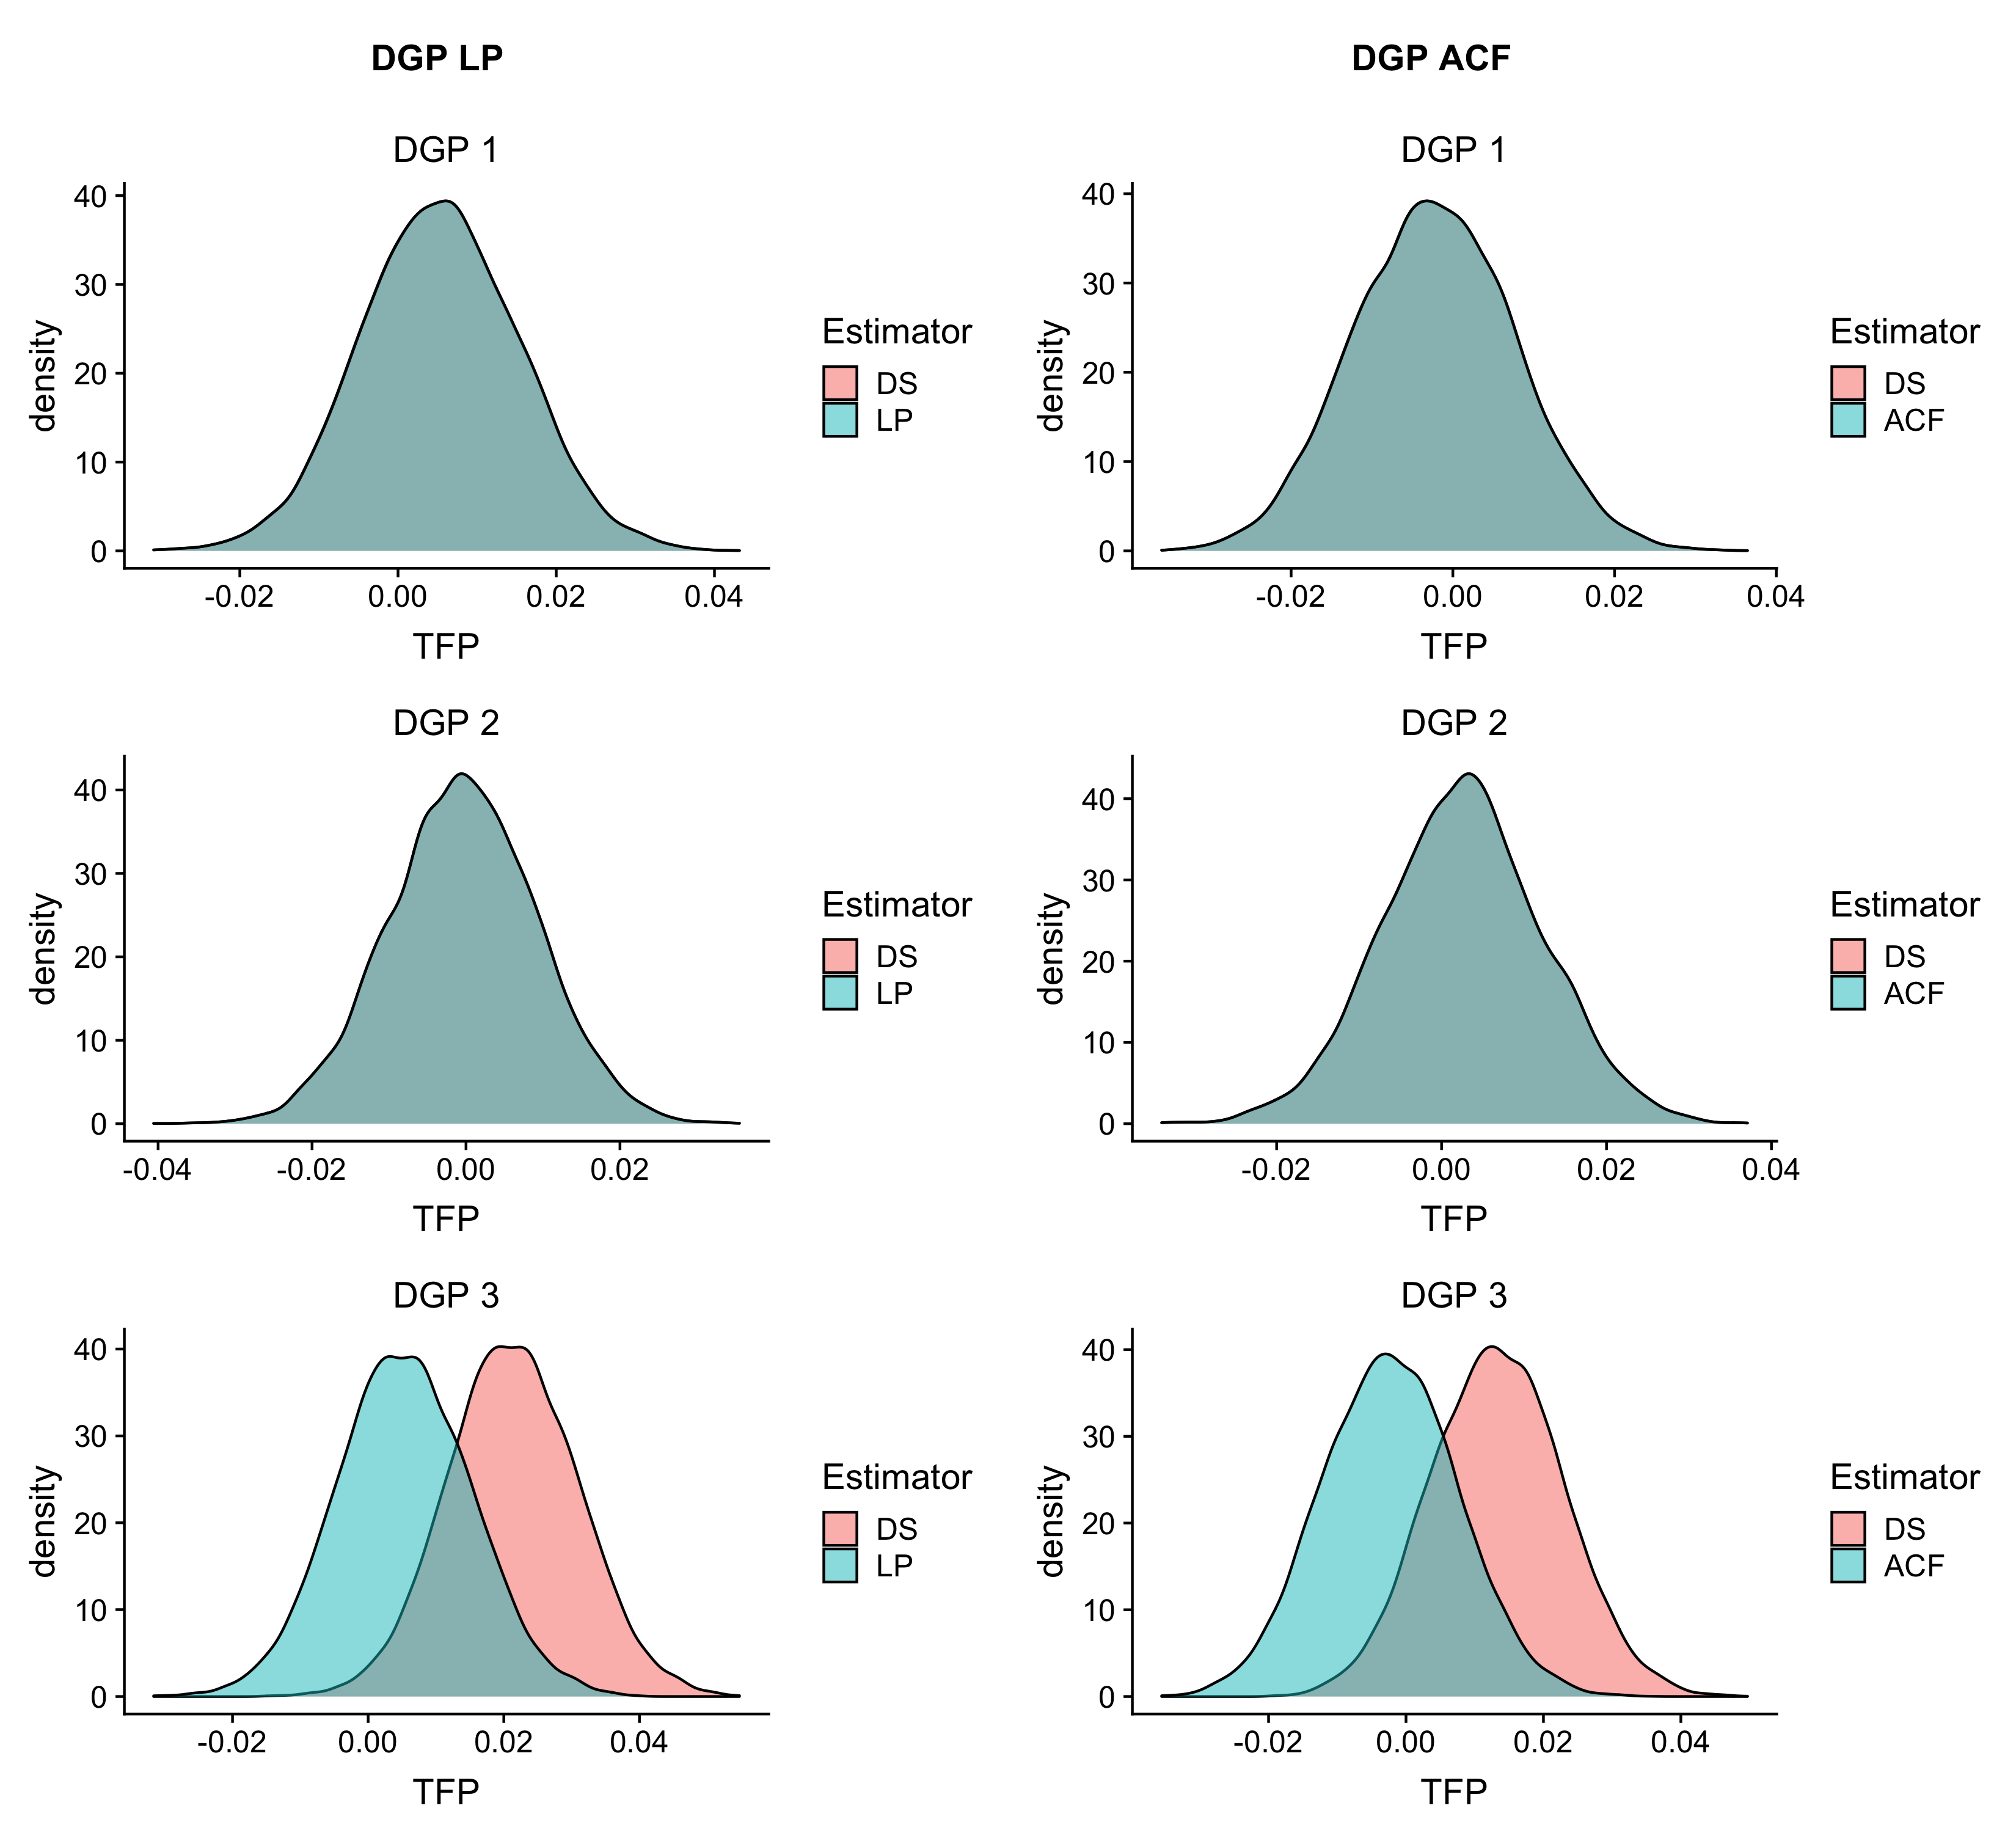
\includegraphics[width=12cm, height=12cm]{/Users/justindoty/Documents/Research/Dissertation/Production_QR_Proxy/Code/Monte_Carlo/TFPplot.png}
\label{fig:MCTFP}
\end{figure}

We are also interested in the differences in Total Factor Productivity (TFP) at the median and the mean. For Figure \ref{fig:MCTFP} we plot densities of TFP using our method and the method of LP and ACF. It is clear for the first two rows DGP1 and DGP2 produce equivalent estimates of TFP since the error distribution was specified as symmetric (Normal for DGP1 and Student-t for DGP2). In DGP3, where the error distribution was specified as log-normal, there are differences between the two estimates. This implies that when the distribution of production shocks are skewed, as is often the case in empirical applications, the median estimate of TFP will be robust to outliers. 

\section{Application} \label{application}
We apply our estimator to popular plant level manufacturing datasets from Chile and Colombia to examine heterogeneity in the output distribution. For both countries, we examine estimates across different manufacturing industries as well as how these estimates have changed over time. We use the DS estimator presented in this paper and compare it to the ACF estimates. We also compare our estimates to the quantile regression estimates without controlling for productivity. In the ACF estimation procedure, we estimate the function $\Phi$ with a 3rd degree polynomial with interactions in capital, labor and materials. To estimate the coefficient on capital and labor, we use the ACF criterion function mentioned earlier. Since we only need a consistent estimator of the production function parameters, we do not consider any over-identification conditions in this step. We use bootstrap to estimate standard errors of $\beta_{k}(\tau)$ and $\beta_{l}(\tau)$ with the number of iterations set to $500$.
%----------------------------------------------------------------------------------------

\subsection{Chilean Manufacturing}
This data comes from the census of Chilean manufacturing plants conducted by the Instituto Nacional de Estadist\'ica (INE). The sample is collected between 1979 and 1996 for firms with more than 10 employees. We divide our estimates into the three largest manufacturing industries: Food (ISIC 311), Fabricated Metals (ISIC 381), and Textiles (ISIC 321). We also aggregate the three industries with the other smaller industries to obtain estimates from the entire sample. Summary statistics for the data we use are provided in Table \ref{CHLsum}.

Figures \ref{fig:ACFCHL311}, \ref{fig:ACFCHL381} and \ref{fig:ACFCHL321} illustrate our estimates from our model compared to ACF estimates as well as their differences to QR estimates. In each industry and the combined sample, estimates of capital elasticity are increasing in firm size. In ISIC 311 and ISIC 381, our model estimates lower capital elasticities than the ACF estimate for small $\tau$. In ISIC 321 and the combined sample, there are differences between these estimates for both small and large $\tau$. The labor estimates in ISIC 311 are increasing but not different from the the ACF estimator. In ISIC 381, labor estimates are are mostly constant and not different from the ACF estimator. In ISIC 381, labor estimates are decreasing but not different from the ACF estimator. Finally, in the combined sample, our estimator is mostly constant and not different from the ACF estimator. Comparing our estimator and QR estimates, we find that there are differences in the estimates for capital and some evidence of differences in labor for small $\tau$ in ISIC 311, 381, and the combined sample. From Table \ref{CHLestACF}, returns to scale are increasing with firm size. Capital intensity is increasing as well except for large firms at $\tau=0.9$ in ISIC 311.

Figure \ref{fig:ACFCHLpgrowth} reports average productivity for all Chilean plants in the sample with base period set to 100. Productivity decreases in the beginning of the 1980s but then increases for the rest of the sample period. These estimates suggest that small firms had higher productivity than large firms. The ACF estimates are similar to productivity of medium-sized firms at $\tau=0.5$. Figure \ref{fig:ACFCHLtimecoef} shows the time trends in output elasticities. The estimates for capital and labor elasticities follow similar trends for each quantile. Capital estimates decrease in the beginning of the sample period then increase, reaching their peak before 1990. These estimates increase in $\tau$. Labor estimates are not much different across quantiles and decrease over time.

\begin{figure}[H]
\centering
\caption{Estimated Coefficients of Capital and Labor for Chile: ISIC 311}
\includegraphics[width=9cm, height=9cm]{/Users/justindoty/Documents/Research/Dissertation/Production_QR_Proxy/Code/Empirical/Chile/Plots/Coefficients/ACF/QACF_Coef_Plot_ISIC_311.png}
\label{fig:ACFCHL311}
\end{figure}

\begin{figure}[H]
\centering
\caption{Estimated Coefficients of Capital and Labor for Chile: ISIC 381}
\includegraphics[width=9cm, height=9cm]{/Users/justindoty/Documents/Research/Dissertation/Production_QR_Proxy/Code/Empirical/Chile/Plots/Coefficients/ACF/QACF_Coef_Plot_ISIC_381.png}
\label{fig:ACFCHL381}
\end{figure}

\begin{figure}[H]
\centering
\caption{Estimated Coefficients of Capital and Labor for Chile: ISIC 321}
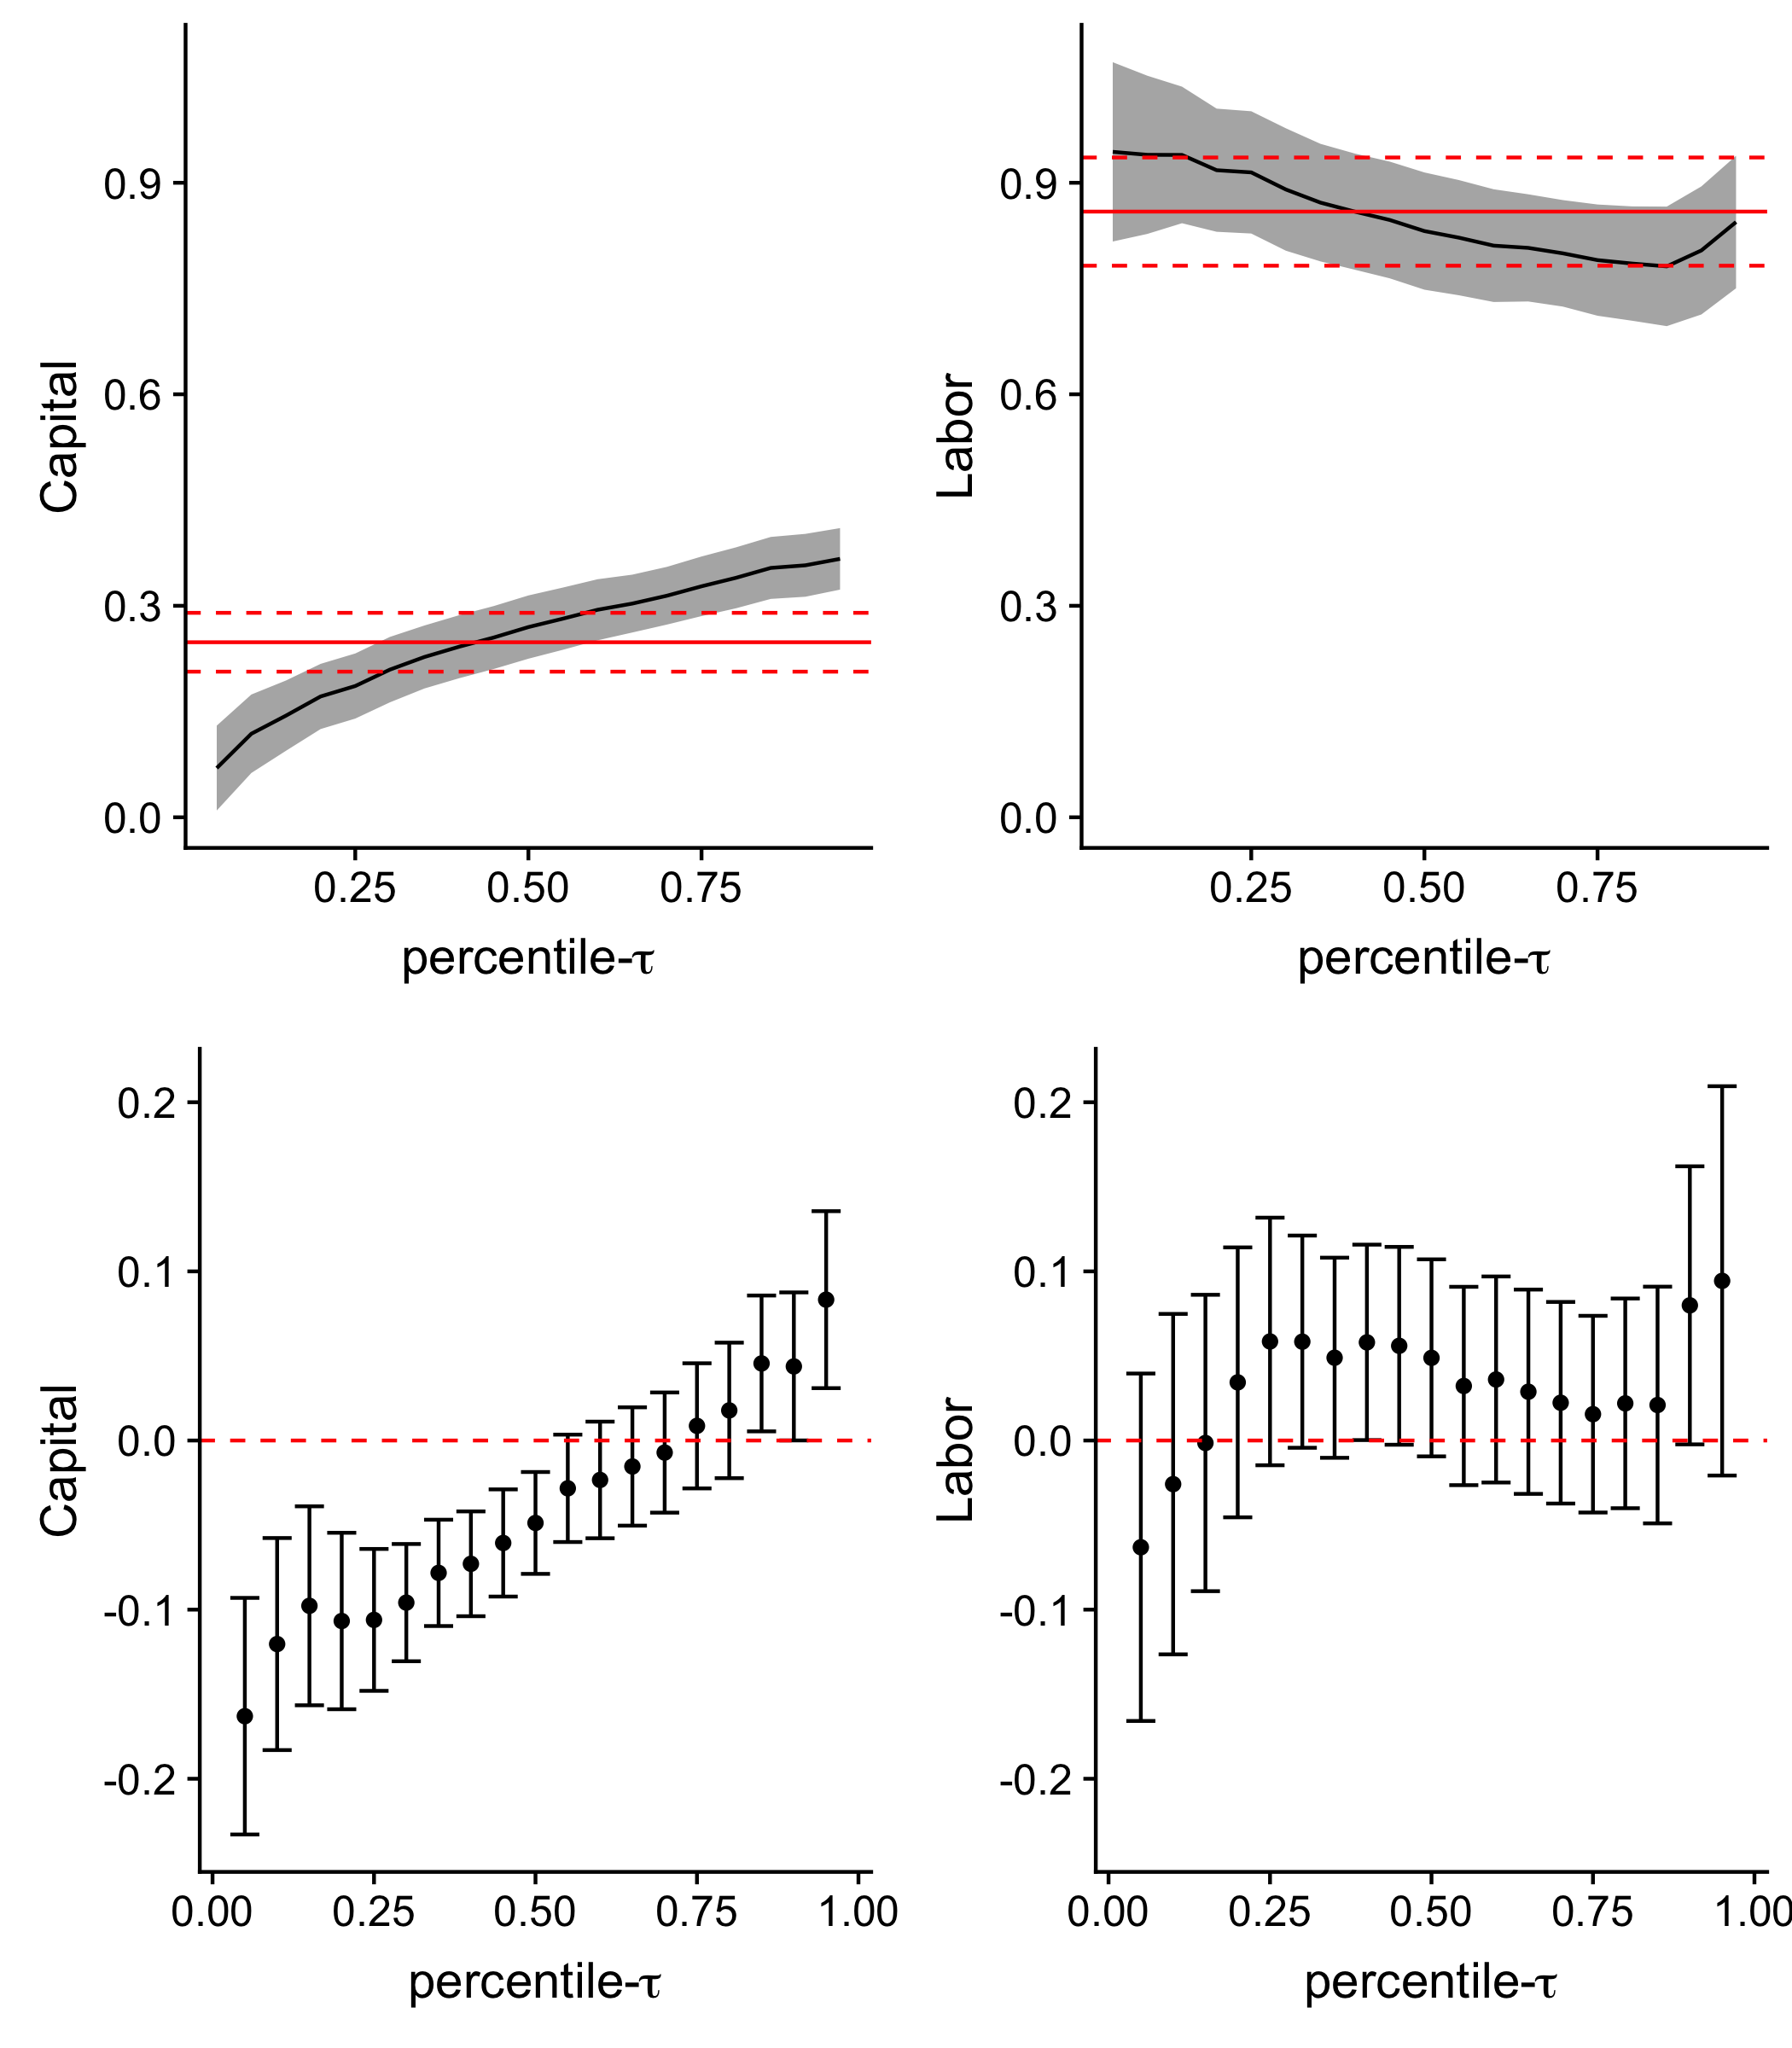
\includegraphics[width=9cm, height=9cm]{/Users/justindoty/Documents/Research/Dissertation/Production_QR_Proxy/Code/Empirical/Chile/Plots/Coefficients/ACF/QACF_Coef_Plot_ISIC_321.png}
\label{fig:ACFCHL321}
\end{figure}

\begin{figure}[H]
\centering
\caption{Estimated Coefficients of Capital and Labor for all Chilean Manufacturing Plants}
\includegraphics[width=9cm, height=9cm]{/Users/justindoty/Documents/Research/Dissertation/Production_QR_Proxy/Code/Empirical/Chile/Plots/Coefficients/ACF/QACF_Coef_Plot_ISIC_All.png}
\label{fig:ACFCHLall}
\end{figure}

\begin{table}[H]
\centering
\caption{Coefficient Estimates and Standard Errors for Chilean Manufacturing Plants}
\begin{tabular}{cccccccccc}
  \hline\hline & & \multicolumn{2}{c}{Capital}  & \multicolumn{2}{c}{Labor} & \multicolumn{2}{c}{Returns to Scale} & \multicolumn{2}{c}{Capital Intensity}\\ \cmidrule(lr){3-4} \cmidrule(lr){5-6} \cmidrule(lr){7-8} \cmidrule(lr){9-10}ISIC & $\tau$ & Coef. & s.e & Coef. & s.e & Coef. & s.e & Coef. & s.e \\ 
  \hline
311 & 0.10 & 0.147 & 0.0211 & 0.721 & 0.0463 & 0.868 & 0.0348 & 0.204 & 0.0408 \\ 
   & 0.25 & 0.199 & 0.0187 & 0.761 & 0.0394 & 0.960 & 0.0315 & 0.262 & 0.0351 \\ 
   & 0.50 & 0.251 & 0.0179 & 0.776 & 0.0342 & 1.028 & 0.0282 & 0.324 & 0.0333 \\ 
   & 0.90 & 0.296 & 0.0195 & 0.898 & 0.0417 & 1.194 & 0.0324 & 0.330 & 0.0343 \\ 
  381 & 0.10 & 0.145 & 0.0294 & 0.920 & 0.0611 & 1.065 & 0.0418 & 0.157 & 0.0411 \\ 
   & 0.25 & 0.216 & 0.0253 & 0.880 & 0.0510 & 1.096 & 0.0366 & 0.245 & 0.0403 \\ 
   & 0.50 & 0.275 & 0.0253 & 0.846 & 0.0505 & 1.121 & 0.0360 & 0.325 & 0.0464 \\ 
   & 0.90 & 0.354 & 0.0284 & 0.848 & 0.0557 & 1.201 & 0.0375 & 0.417 & 0.0568 \\ 
  321 & 0.10 & 0.119 & 0.0338 & 0.940 & 0.0682 & 1.058 & 0.0442 & 0.126 & 0.0435 \\ 
   & 0.25 & 0.186 & 0.0281 & 0.915 & 0.0527 & 1.101 & 0.0367 & 0.204 & 0.0420 \\ 
   & 0.50 & 0.270 & 0.0273 & 0.831 & 0.0505 & 1.101 & 0.0358 & 0.324 & 0.0498 \\ 
   & 0.90 & 0.357 & 0.0271 & 0.804 & 0.0552 & 1.161 & 0.0401 & 0.445 & 0.0614 \\ 
  All & 0.10 & 0.194 & 0.0115 & 0.828 & 0.0233 & 1.022 & 0.0155 & 0.234 & 0.0198 \\ 
   & 0.25 & 0.268 & 0.0098 & 0.810 & 0.0181 & 1.078 & 0.0128 & 0.330 & 0.0182 \\ 
   & 0.50 & 0.339 & 0.0091 & 0.771 & 0.0154 & 1.110 & 0.0111 & 0.439 & 0.0190 \\ 
   & 0.90 & 0.418 & 0.0103 & 0.806 & 0.0190 & 1.224 & 0.0129 & 0.519 & 0.0237 \\ 
   \hline
\end{tabular}
\caption*{\footnotesize $^{*}$Standard errors are obtained using bootstrap with 500 replications. Productivity is estimated using ACF}
\label{CHLestACF}
\end{table}

\begin{figure}[H]
\centering
\caption{Mean and Median Estimates of Total Factor Productivity}
\includegraphics[width=12cm]{/Users/justindoty/Documents/Research/Dissertation/Production_QR_Proxy/Code/Empirical/Chile/Plots/TFP/QACF_TFP_Plot.png}
\label{fig:ACFCHLTFPDens}
\end{figure}

\begin{figure}[H]
\centering
\caption{Chile Productivity Over Time}
\includegraphics[width=12cm]{/Users/justindoty/Documents/Research/Dissertation/Production_QR_Proxy/Code/Empirical/Chile/Plots/TFP/QACF_TFPgrowth_Plot.png}
\label{fig:ACFCHLpgrowth}
\end{figure}



%------------------------------------------------------------------------------------------------

\subsection{Colombian Manufacturing}
This data comes from the Colombian manufacturing census conducted by the Departamento Administrativo Nacional de Estadistica. The sample is collected between 1977 and 1991. We divide our estimates into the three largest manufacturing industries: Food (ISIC 311), Apparel (ISIC 322), and Fabricated Metals (ISIC 381). As we did with the Chilean sample, we also aggregate the three industries with other smaller industries to obtain estimates from the entire sample of manufacturing plants. Summary statistics for this data is provided in Table \ref{COLsum}.

Figures \ref{fig:ACFCOL311}, \ref{fig:ACFCOL321}, and \ref{fig:ACFCOL381} illustrate estimates from our model compared to the ACF estimates as well as their differences from QR estimates. The capital estimates in each industry are increasing and are significantly different than the ACF estimates. The labor estimates in each industry are decreasing, however, only in the combined sample are these estimates different from ACF for both low and high $\tau$. Comparing our results to those obtained using QR, there is statistical difference in ISIC 311, difference in the labor estimate in ISIC 321 and ISIC 381 and differences in both capital and labor in the combined sample.

\begin{figure}[H]
\centering
\caption{Estimated Coefficients of Capital and Labor for Colombia: ISIC 311}
\includegraphics[width=9cm, height=9cm]{/Users/justindoty/Documents/Research/Dissertation/Production_QR_Proxy/Code/Empirical/Colombia/Plots/Coefficients/ACF/QACF_Coef_Plot_ISIC_311.png}
\label{fig:ACFCOL311}
\end{figure}

\begin{figure}[H]
\centering
\caption{Estimated Coefficients of Capital and Labor for Colombia: ISIC 321}
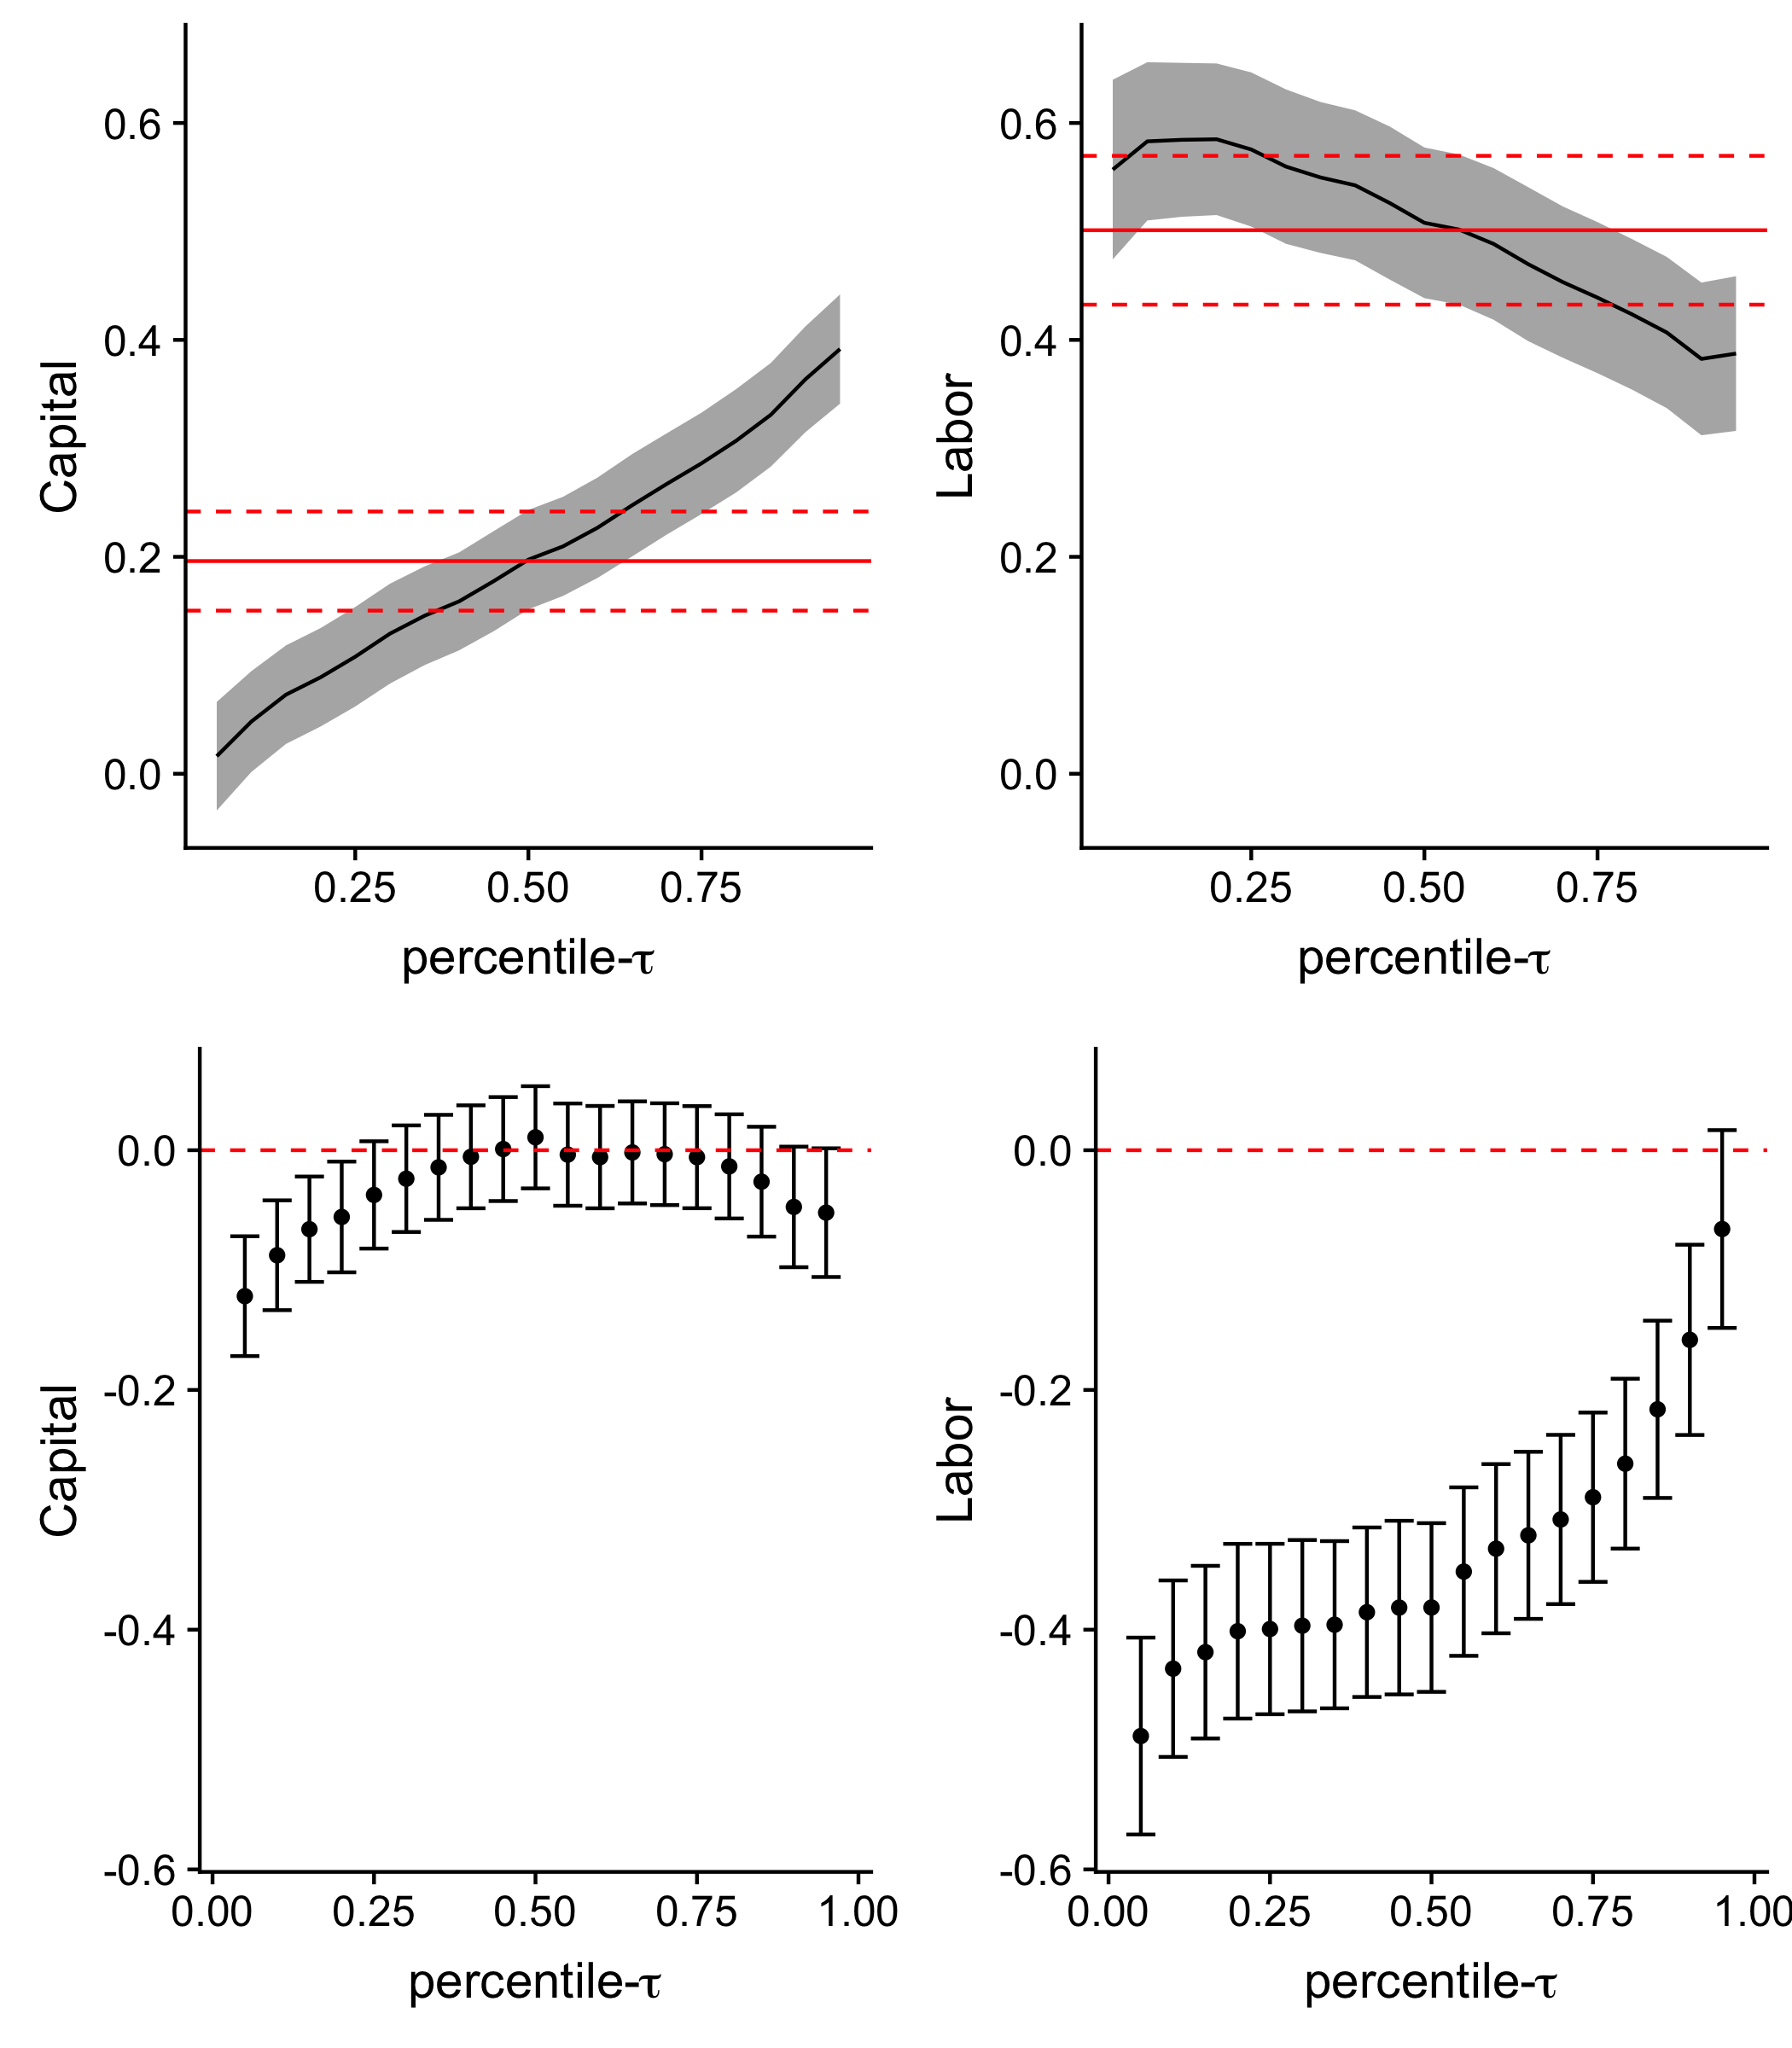
\includegraphics[width=9cm, height=9cm]{/Users/justindoty/Documents/Research/Dissertation/Production_QR_Proxy/Code/Empirical/Colombia/Plots/Coefficients/ACF/QACF_Coef_Plot_ISIC_322.png}
\label{fig:ACFCOL321}
\end{figure}

\begin{figure}[H]
\centering
\caption{Estimated Coefficients of Capital and Labor for Colombia: ISIC 381}
\includegraphics[width=9cm, height=9cm]{/Users/justindoty/Documents/Research/Dissertation/Production_QR_Proxy/Code/Empirical/Colombia/Plots/Coefficients/ACF/QACF_Coef_Plot_ISIC_381.png}
\label{fig:ACFCOL381}
\end{figure}

\begin{figure}[H]
\centering
\caption{Estimated Coefficients of Capital and Labor for all Colombian Manufacturing Plants}
\includegraphics[width=9cm, height=9cm]{/Users/justindoty/Documents/Research/Dissertation/Production_QR_Proxy/Code/Empirical/Colombia/Plots/Coefficients/ACF/QACF_Coef_Plot_ISIC_All.png}
\label{fig:ACFCOLall}
\end{figure}

Using these estimates we construct measures of returns to scale and capital intensity for each industry in Table \ref{COLestACF}. Most firms experience constant or slightly decreasing returns to scale. Returns to scale are smallest in ISIC 311. Returns to scale and capital intensity are increasing in firm size.

\begin{table}[H]
\centering
\caption{Coefficient Estimates and Standard Errors for Colombian Manufacturing Plants}
\begin{tabular}{cccccccccc}
  \hline\hline & & \multicolumn{2}{c}{Capital}  & \multicolumn{2}{c}{Labor} & \multicolumn{2}{c}{Returns to Scale} & \multicolumn{2}{c}{Capital Intensity}\\ \cmidrule(lr){3-4} \cmidrule(lr){5-6} \cmidrule(lr){7-8} \cmidrule(lr){9-10}ISIC & $\tau$ & Coef. & s.e & Coef. & s.e & Coef. & s.e & Coef. & s.e \\ 
  \hline
311 & 0.10 & 0.085 & 0.0217 & 0.649 & 0.0505 & 0.735 & 0.0448 & 0.131 & 0.0376 \\ 
   & 0.25 & 0.156 & 0.0201 & 0.622 & 0.0448 & 0.777 & 0.0419 & 0.251 & 0.0395 \\ 
   & 0.50 & 0.231 & 0.0201 & 0.563 & 0.0438 & 0.795 & 0.0412 & 0.411 & 0.0503 \\ 
   & 0.90 & 0.398 & 0.0230 & 0.423 & 0.0496 & 0.822 & 0.0429 & 0.942 & 0.1251 \\ 
  322 & 0.10 & 0.048 & 0.0283 & 0.583 & 0.0444 & 0.631 & 0.0413 & 0.083 & 0.0504 \\ 
   & 0.25 & 0.108 & 0.0279 & 0.576 & 0.0432 & 0.683 & 0.0407 & 0.187 & 0.0549 \\ 
   & 0.50 & 0.197 & 0.0279 & 0.508 & 0.0422 & 0.705 & 0.0401 & 0.389 & 0.0718 \\ 
   & 0.90 & 0.364 & 0.0296 & 0.382 & 0.0428 & 0.746 & 0.0394 & 0.951 & 0.1509 \\ 
  381 & 0.10 & 0.151 & 0.0363 & 0.904 & 0.0589 & 1.055 & 0.0472 & 0.167 & 0.0487 \\ 
   & 0.25 & 0.240 & 0.0329 & 0.863 & 0.0426 & 1.102 & 0.0401 & 0.278 & 0.0472 \\ 
   & 0.50 & 0.341 & 0.0345 & 0.763 & 0.0435 & 1.104 & 0.0391 & 0.447 & 0.0640 \\ 
   & 0.90 & 0.478 & 0.0385 & 0.680 & 0.0498 & 1.159 & 0.0389 & 0.703 & 0.0975 \\ 
  All & 0.10 & 0.105 & 0.0101 & 0.737 & 0.0214 & 0.843 & 0.0186 & 0.143 & 0.0156 \\ 
   & 0.25 & 0.189 & 0.0095 & 0.710 & 0.0198 & 0.899 & 0.0179 & 0.266 & 0.0173 \\ 
   & 0.50 & 0.268 & 0.0096 & 0.660 & 0.0197 & 0.928 & 0.0177 & 0.406 & 0.0215 \\ 
   & 0.90 & 0.417 & 0.0105 & 0.571 & 0.0209 & 0.988 & 0.0179 & 0.730 & 0.0368 \\ 
   \hline
\end{tabular}
\caption*{\footnotesize $^{*}$Standard errors are obtained using bootstrap with 500 replications. Productivity is estimated using ACF}
\label{COLestACF}
\end{table}

Figure \ref{fig:ACFCOACFgrowth} reports average productivity for all Colombian plants in the sample with base period set to 100. Productivity decreases in the beginning of the sample period, but then increases for the rest of the sample period after 1980 with some periods of sharp changes. Each percentile of firm size has similar productivity levels throughout the sample period. Figure \ref{fig:ACFCOLtimecoef} shows the time trends in output elasticities. Capital estimates are generally increases except for a slight dip in 1985. These estimates are increasing in $\tau$. The estimates of labor elasticity are similar in the beginning of the sample period. They increase past 1980 where dispersion across quantiles is largest, then decrease and dispersion lessens.

\begin{figure}[H]
\centering
\caption{Mean and Median Estimates of Total Factor Productivity}
\includegraphics[width=12cm]{/Users/justindoty/Documents/Research/Dissertation/Production_QR_Proxy/Code/Empirical/Colombia/Plots/TFP/QACF_TFP_Plot.png}
\label{fig:ACFCOLTFPDens}
\end{figure}

\begin{figure}[H]
\centering
\caption{Chile Productivity Over Time}
\includegraphics[width=12cm]{/Users/justindoty/Documents/Research/Dissertation/Production_QR_Proxy/Code/Empirical/Colombia/Plots/TFP/QACF_TFPgrowth_Plot.png}
\label{fig:ACFCOLpgrowth}
\end{figure}

\section{Conclusions} \label{conclusion}

We propose a method that extends the proxy variable approach to estimating the conditional quantiles of firm size. The method is computationally attractive as it resembles the two-stage estimator proposed by \cite{Canay2011}. As a result, practitioners are able to easily apply the proposed estimator to production function models where the data may reveal significant heterogeneous output elasticities along the conditional firm size distribution. We showed that this estimator works well in finite samples and showed that it captures heterogeneity in firm size under different data generating processes. An application to widely used datasets from the US, Chile, and Colombia showed that in some industries, our estimator captures unobserved heterogeneity that the LP estimator does not.

Improvements and extensions of this estimator are currently being explored. For example, using a value-added production function may show more heterogeneity in estimates of elasticities and productivity than a gross-output production function. However, using a gross-output production function with an intermediate input proxy variable suffers from non-identification. We are currently working on an identification strategy that allows for different types of production function estimators such as the one proposed by \cite{Gandhi2020}. This paper also makes an interesting but brief connection between the literature on production risk and quantile utility maximization. Currently, quantile utility maximization problems and estimation of these models are being studied by \cite{Castro2017} and \cite{qgmm} in the context of dynamic consumption problems. It would be interesting to explore a model for a firm who maximizes quantile utility of profits which could provide an alternative interpretation for unobserved heterogeneity that are obtained from quantile regression estimates.

This paper contributes to the growing literature on production functions with unobserved heterogeneity. We show that differences in firm size correspond to the the rank of the ex-post shock. The location-shift model for productivity we propose here restricts us from examining other dimensions of firm heterogeneity. Therefore, allowing richer distributional effects of productivity would be an interesting extension. This approach also restricts us from examining non-Hicks neutral productivity shocks such as factor-augmenting productivity. We are currently working on an extension of this paper to a non-separable model to address these last two points, but the estimator we propose here is computationally attractive and easy to implement in empirical research.    




\pagebreak
\newpage



%\section*{Appendix}
%\appendix
%\begin{Large}
%\noindent \textbf{A. Proof of the Theorems}
%\end{Large}

%\counterwithin{theorem}{section}
%\section{Proofs}





\bibliographystyle{ecca.bst}
\bibliography{references}

\section*{Appendix} \label{Appendix}
\subsection{Summary Statistics}
\subsubsection{US}
\begin{table}[H]
\centering
\caption{Summary Statistics (in logs) for US Manufacturing Data}
\begin{tabular}{ccccccc}
  \hline\hline Industry (NAICS code) &   & 1st Qu. & Median & 3rd Qu. & Mean & sd \\ 
  \hline
31 (Total=3271) & Output & 19.05 & 20.24 & 21.57 & 20.3 & 1.77 \\ 
   & Capital & 18.66 & 20.37 & 21.76 & 20.19 & 2.12 \\ 
   & Labor & 17.42 & 19.08 & 20.61 & 19.02 & 2.21 \\ 
   & Materials & 17.96 & 19.59 & 21.15 & 19.54 & 2.21 \\ 
  32 (Total=7207) & Output & 15.67 & 17.04 & 18.51 & 17.01 & 2.05 \\ 
   & Capital & 15.65 & 17.51 & 19.13 & 17.31 & 2.41 \\ 
   & Labor & 14.44 & 16.01 & 17.57 & 16.01 & 2.29 \\ 
   & Materials & 14.89 & 16.53 & 18.25 & 16.52 & 2.37 \\ 
  33 (Total=13978) & Output & 7.38 & 8.58 & 9.8 & 8.5 & 1.67 \\ 
   & Capital & 6.67 & 8.29 & 9.74 & 8.15 & 1.95 \\ 
   & Labor & 6.01 & 7.42 & 8.91 & 7.48 & 1.93 \\ 
   & Materials & 6.33 & 7.82 & 9.29 & 7.82 & 1.95 \\ 
  All (Total=24456) & Output & 18.58 & 19.78 & 21.23 & 19.85 & 1.79 \\ 
   & Capital & 18.14 & 19.86 & 21.26 & 19.67 & 2.16 \\ 
   & Labor & 16.98 & 18.59 & 20.13 & 18.56 & 2.17 \\ 
   & Materials & 17.49 & 19.12 & 20.66 & 19.06 & 2.2 \\ 
   \hline
\end{tabular}
\label{USsum}
\end{table}

\subsubsection{Chile}

\begin{table}[H]
\centering
\caption{Summary Statistics (in logs) for Chilean Manufacturing Plants}
\begin{tabular}{ccccccc}
  \hline\hline Industry (ISIC code) &   & 1st Qu. & Median & 3rd Qu. & Mean & sd \\ 
  \hline
311 (Total=13838) & Output & 10.21 & 10.84 & 12.22 & 11.36 & 1.58 \\ 
   & Capital & 10.56 & 11.4 & 12.4 & 11.52 & 1.37 \\ 
   & Labor & 10.49 & 11.4 & 12.54 & 11.53 & 1.43 \\ 
   & Materials & 10.38 & 11.28 & 12.53 & 11.56 & 1.6 \\ 
  381 (Total=4311) & Output & 6.69 & 7.66 & 9.06 & 8.02 & 1.98 \\ 
   & Capital & 7.52 & 8.51 & 9.7 & 8.65 & 1.68 \\ 
   & Labor & 7.21 & 8.34 & 9.56 & 8.4 & 1.72 \\ 
   & Materials & 7.22 & 8.35 & 9.72 & 8.54 & 1.92 \\ 
  321 (Total=4302) & Output & 2.77 & 3.22 & 3.91 & 3.49 & 0.99 \\ 
   & Capital & 2.89 & 3.47 & 4.22 & 3.71 & 1.08 \\ 
   & Labor & 2.94 & 3.48 & 4.37 & 3.69 & 0.95 \\ 
   & Materials & 2.89 & 3.43 & 4.28 & 3.67 & 1.02 \\ 
  All (Total=51567) & Output & 9.84 & 10.46 & 11.81 & 10.94 & 1.56 \\ 
   & Capital & 9.91 & 10.75 & 11.79 & 10.86 & 1.41 \\ 
   & Labor & 9.68 & 10.62 & 11.75 & 10.73 & 1.48 \\ 
   & Materials & 9.81 & 10.68 & 11.89 & 10.93 & 1.62 \\ 
   \hline
\end{tabular}
\label{CHLsum}
\end{table} 

\subsubsection{Colombia}

\begin{table}[H]
\centering
\caption{Summary Statistics (in logs) for Colombian Manufacturing Plants}
\begin{tabular}{ccccccc}
  \hline\hline Industry (ISIC code) &   & 1st Qu. & Median & 3rd Qu. & Mean & sd \\ 
  \hline
311 (Total=13215) & Output & 9.03 & 10.21 & 11.59 & 10.42 & 1.8 \\ 
   & Capital & 8.69 & 9.37 & 10.22 & 9.49 & 1.18 \\ 
   & Labor & 8.52 & 9.3 & 10.33 & 9.54 & 1.43 \\ 
   & Materials & 8.7 & 9.62 & 10.88 & 9.92 & 1.67 \\ 
  322 (Total=12182) & Output & 6.02 & 7.07 & 8.35 & 7.24 & 1.78 \\ 
   & Capital & 5.47 & 6.14 & 6.93 & 6.23 & 1.21 \\ 
   & Labor & 5.89 & 6.75 & 7.81 & 6.93 & 1.55 \\ 
   & Materials & 5.9 & 6.89 & 8.16 & 7.12 & 1.77 \\ 
  381 (Total=7411) & Output & 2.56 & 3.09 & 3.97 & 3.36 & 1.1 \\ 
   & Capital & 2.77 & 3.3 & 3.95 & 3.42 & 0.92 \\ 
   & Labor & 2.64 & 3.18 & 3.91 & 3.37 & 0.98 \\ 
   & Materials & 2.71 & 3.3 & 4.11 & 3.5 & 1.09 \\ 
  All (Total=87783) & Output & 8.39 & 9.73 & 11.26 & 9.87 & 2 \\ 
   & Capital & 7.62 & 8.53 & 9.46 & 8.48 & 1.51 \\ 
   & Labor & 7.77 & 8.65 & 9.72 & 8.8 & 1.58 \\ 
   & Materials & 7.89 & 8.93 & 10.26 & 9.15 & 1.88 \\ 
   \hline
\end{tabular}
\label{COLsum}
\end{table}

\subsection{Estimates using \cite{Levinsohn2003}}

\subsubsection{Chile}

\begin{table}[H]
\centering
\caption{Coefficient Estimates and Standard Errors for Chilean Manufacturing Plants}
\begin{tabular}{cccccccccc}
  \hline\hline & & \multicolumn{2}{c}{Capital}  & \multicolumn{2}{c}{Labor} & \multicolumn{2}{c}{Returns to Scale} & \multicolumn{2}{c}{Capital Intensity}\\ \cmidrule(lr){3-4} \cmidrule(lr){5-6} \cmidrule(lr){7-8} \cmidrule(lr){9-10}ISIC & $\tau$ & Coef. & s.e & Coef. & s.e & Coef. & s.e & Coef. & s.e \\ 
  \hline
311 & 0.10 & 0.195 & 0.0225 & 0.356 & 0.0365 & 0.552 & 0.0304 & 0.548 & 0.1100 \\ 
   & 0.25 & 0.245 & 0.0204 & 0.403 & 0.0271 & 0.648 & 0.0265 & 0.607 & 0.0767 \\ 
   & 0.50 & 0.302 & 0.0195 & 0.406 & 0.0219 & 0.707 & 0.0243 & 0.744 & 0.0720 \\ 
   & 0.90 & 0.335 & 0.0202 & 0.551 & 0.0326 & 0.887 & 0.0300 & 0.608 & 0.0610 \\ 
  381 & 0.10 & 0.232 & 0.0299 & 0.651 & 0.0583 & 0.883 & 0.0442 & 0.356 & 0.0771 \\ 
   & 0.25 & 0.305 & 0.0251 & 0.606 & 0.0424 & 0.911 & 0.0371 & 0.503 & 0.0673 \\ 
   & 0.50 & 0.372 & 0.0248 & 0.553 & 0.0382 & 0.926 & 0.0345 & 0.673 & 0.0791 \\ 
   & 0.90 & 0.437 & 0.0293 & 0.586 & 0.0536 & 1.023 & 0.0410 & 0.745 & 0.1118 \\ 
  321 & 0.10 & 0.156 & 0.0358 & 0.709 & 0.0638 & 0.864 & 0.0462 & 0.220 & 0.0687 \\ 
   & 0.25 & 0.239 & 0.0301 & 0.648 & 0.0444 & 0.887 & 0.0378 & 0.369 & 0.0659 \\ 
   & 0.50 & 0.319 & 0.0291 & 0.573 & 0.0417 & 0.892 & 0.0368 & 0.556 & 0.0824 \\ 
   & 0.90 & 0.404 & 0.0300 & 0.554 & 0.0452 & 0.957 & 0.0386 & 0.729 & 0.1073 \\ 
  All & 0.10 & 0.222 & 0.0113 & 0.500 & 0.0227 & 0.722 & 0.0170 & 0.444 & 0.0393 \\ 
   & 0.25 & 0.301 & 0.0100 & 0.466 & 0.0171 & 0.767 & 0.0139 & 0.645 & 0.0400 \\ 
   & 0.50 & 0.371 & 0.0092 & 0.428 & 0.0138 & 0.799 & 0.0122 & 0.868 & 0.0427 \\ 
   & 0.90 & 0.439 & 0.0111 & 0.493 & 0.0196 & 0.932 & 0.0144 & 0.890 & 0.0542 \\ 
   \hline
\end{tabular}
\caption*{\footnotesize Standard errors are obtained using bootstrap with 500 replications. Productivity is estimated using LP.}
\label{CHLestLP}
\end{table}

\begin{figure}[H]
\centering
\caption{Estimated Coefficients of Capital and Labor for Chile: ISIC 311}
\includegraphics[width=9cm, height=9cm]{/Users/justindoty/Documents/Research/Dissertation/Production_QR_Proxy/Code/Empirical/Chile/Plots/Coefficients/LP/QLP_Coef_Plot_ISIC_311.png}
\label{fig:LPCHL311}
\end{figure}

\begin{figure}[H]
\centering
\caption{Estimated Coefficients of Capital and Labor for Chile: ISIC 381}
\includegraphics[width=9cm, height=9cm]{/Users/justindoty/Documents/Research/Dissertation/Production_QR_Proxy/Code/Empirical/Chile/Plots/Coefficients/LP/QLP_Coef_Plot_ISIC_381.png}
\label{fig:LPCHL381}
\end{figure}

\begin{figure}[H]
\centering
\caption{Estimated Coefficients of Capital and Labor for Chile: ISIC 321}
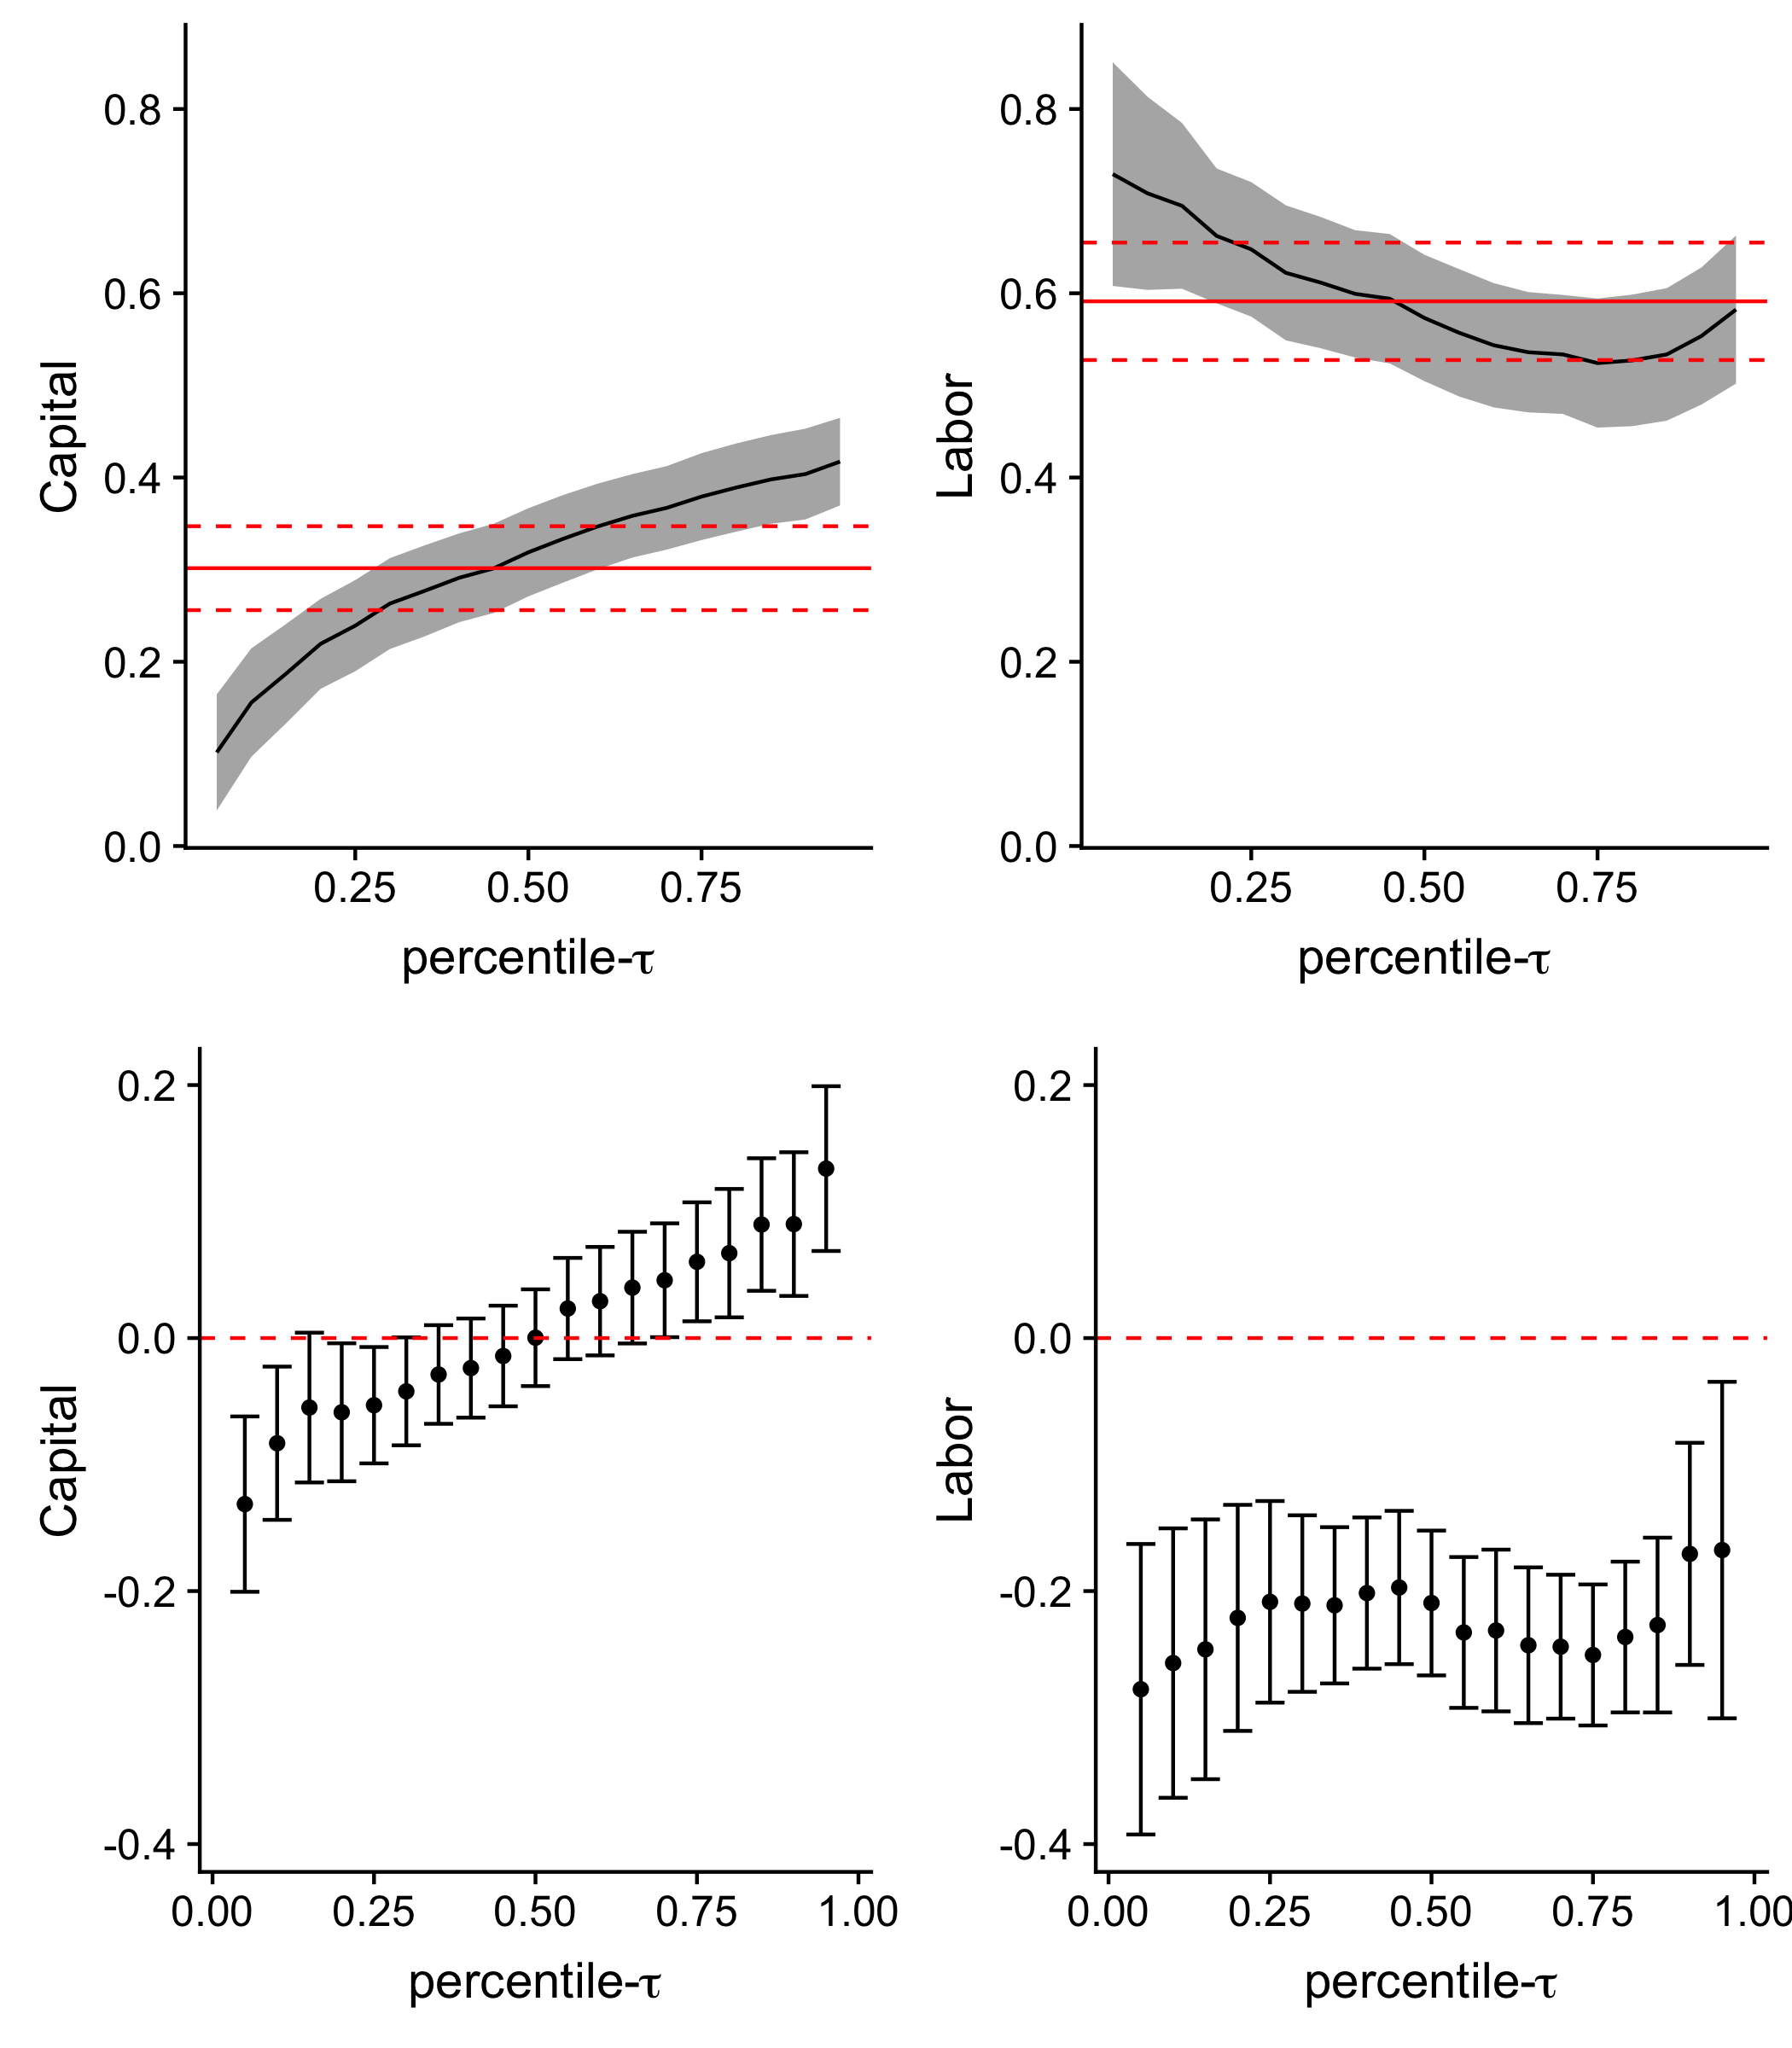
\includegraphics[width=9cm, height=9cm]{/Users/justindoty/Documents/Research/Dissertation/Production_QR_Proxy/Code/Empirical/Chile/Plots/Coefficients/LP/QLP_Coef_Plot_ISIC_321.png}
\label{fig:LPCHL321}
\end{figure}

\begin{figure}[H]
\centering
\caption{Estimated Coefficients of Capital and Labor for all Chilean Manufacturing Plants}
\includegraphics[width=9cm, height=9cm]{/Users/justindoty/Documents/Research/Dissertation/Production_QR_Proxy/Code/Empirical/Chile/Plots/Coefficients/LP/QLP_Coef_Plot_ISIC_All.png}
\label{fig:LPCHLall}
\end{figure}

\begin{figure}[H]
\centering
\caption{Mean and Median Estimates of Total Factor Productivity}
\includegraphics[width=12cm]{/Users/justindoty/Documents/Research/Dissertation/Production_QR_Proxy/Code/Empirical/Chile/Plots/TFP/QLP_TFP_Plot.png}
\label{fig:LPTFPDens}
\end{figure}

\begin{figure}[H]
\centering
\caption{Chile Productivity Over Time}
\includegraphics[width=12cm]{/Users/justindoty/Documents/Research/Dissertation/Production_QR_Proxy/Code/Empirical/Chile/Plots/TFP/QLP_TFPgrowth_Plot.png}
\label{fig:LPCHLpgrowth}
\end{figure}

\subsubsection{Colombia}

\begin{table}[H]
\centering
\caption{Coefficient Estimates and Standard Errors for Colombian Manufacturing Plants}
\begin{tabular}{cccccccccc}
  \hline\hline & & \multicolumn{2}{c}{Capital}  & \multicolumn{2}{c}{Labor} & \multicolumn{2}{c}{Returns to Scale} & \multicolumn{2}{c}{Capital Intensity}\\ \cmidrule(lr){3-4} \cmidrule(lr){5-6} \cmidrule(lr){7-8} \cmidrule(lr){9-10}ISIC & $\tau$ & Coef. & s.e & Coef. & s.e & Coef. & s.e & Coef. & s.e \\ 
  \hline
311 & 0.10 & 0.175 & 0.0278 & 0.618 & 0.0331 & 0.793 & 0.0351 & 0.284 & 0.0520 \\ 
   & 0.25 & 0.237 & 0.0265 & 0.612 & 0.0193 & 0.849 & 0.0299 & 0.387 & 0.0473 \\ 
   & 0.50 & 0.324 & 0.0266 & 0.530 & 0.0172 & 0.854 & 0.0291 & 0.612 & 0.0568 \\ 
   & 0.90 & 0.510 & 0.0281 & 0.354 & 0.0283 & 0.864 & 0.0320 & 1.439 & 0.1609 \\ 
  322 & 0.10 & 0.144 & 0.0242 & 0.683 & 0.0281 & 0.828 & 0.0306 & 0.212 & 0.0387 \\ 
   & 0.25 & 0.202 & 0.0250 & 0.676 & 0.0256 & 0.878 & 0.0286 & 0.299 & 0.0418 \\ 
   & 0.50 & 0.296 & 0.0260 & 0.604 & 0.0274 & 0.899 & 0.0285 & 0.490 & 0.0548 \\ 
   & 0.90 & 0.492 & 0.0322 & 0.441 & 0.0418 & 0.933 & 0.0313 & 1.116 & 0.1645 \\ 
  381 & 0.10 & 0.167 & 0.0385 & 0.933 & 0.0508 & 1.099 & 0.0501 & 0.179 & 0.0448 \\ 
   & 0.25 & 0.265 & 0.0356 & 0.871 & 0.0330 & 1.135 & 0.0442 & 0.304 & 0.0438 \\ 
   & 0.50 & 0.370 & 0.0358 & 0.763 & 0.0306 & 1.132 & 0.0430 & 0.485 & 0.0521 \\ 
   & 0.90 & 0.509 & 0.0397 & 0.678 & 0.0403 & 1.188 & 0.0432 & 0.751 & 0.0822 \\ 
  All & 0.10 & 0.097 & 0.0115 & 0.738 & 0.0136 & 0.836 & 0.0133 & 0.132 & 0.0169 \\ 
   & 0.25 & 0.183 & 0.0108 & 0.706 & 0.0096 & 0.889 & 0.0119 & 0.259 & 0.0169 \\ 
   & 0.50 & 0.266 & 0.0108 & 0.648 & 0.0085 & 0.915 & 0.0115 & 0.411 & 0.0190 \\ 
   & 0.90 & 0.413 & 0.0117 & 0.570 & 0.0117 & 0.983 & 0.0121 & 0.724 & 0.0306 \\ 
   \hline
\end{tabular}
\caption*{\footnotesize Standard errors are obtained using bootstrap with 500 replications. Productivity is estimated using LP.}
\label{COLestLP}
\end{table}

\begin{figure}[H]
\centering
\caption{Estimated Coefficients of Capital and Labor for Colombia: ISIC 311}
\includegraphics[width=9cm, height=9cm]{/Users/justindoty/Documents/Research/Dissertation/Production_QR_Proxy/Code/Empirical/Colombia/Plots/Coefficients/LP/QLP_Coef_Plot_ISIC_311.png}
\label{fig:LPCOL311}
\end{figure}

\begin{figure}[H]
\centering
\caption{Estimated Coefficients of Capital and Labor for Colombia: ISIC 321}
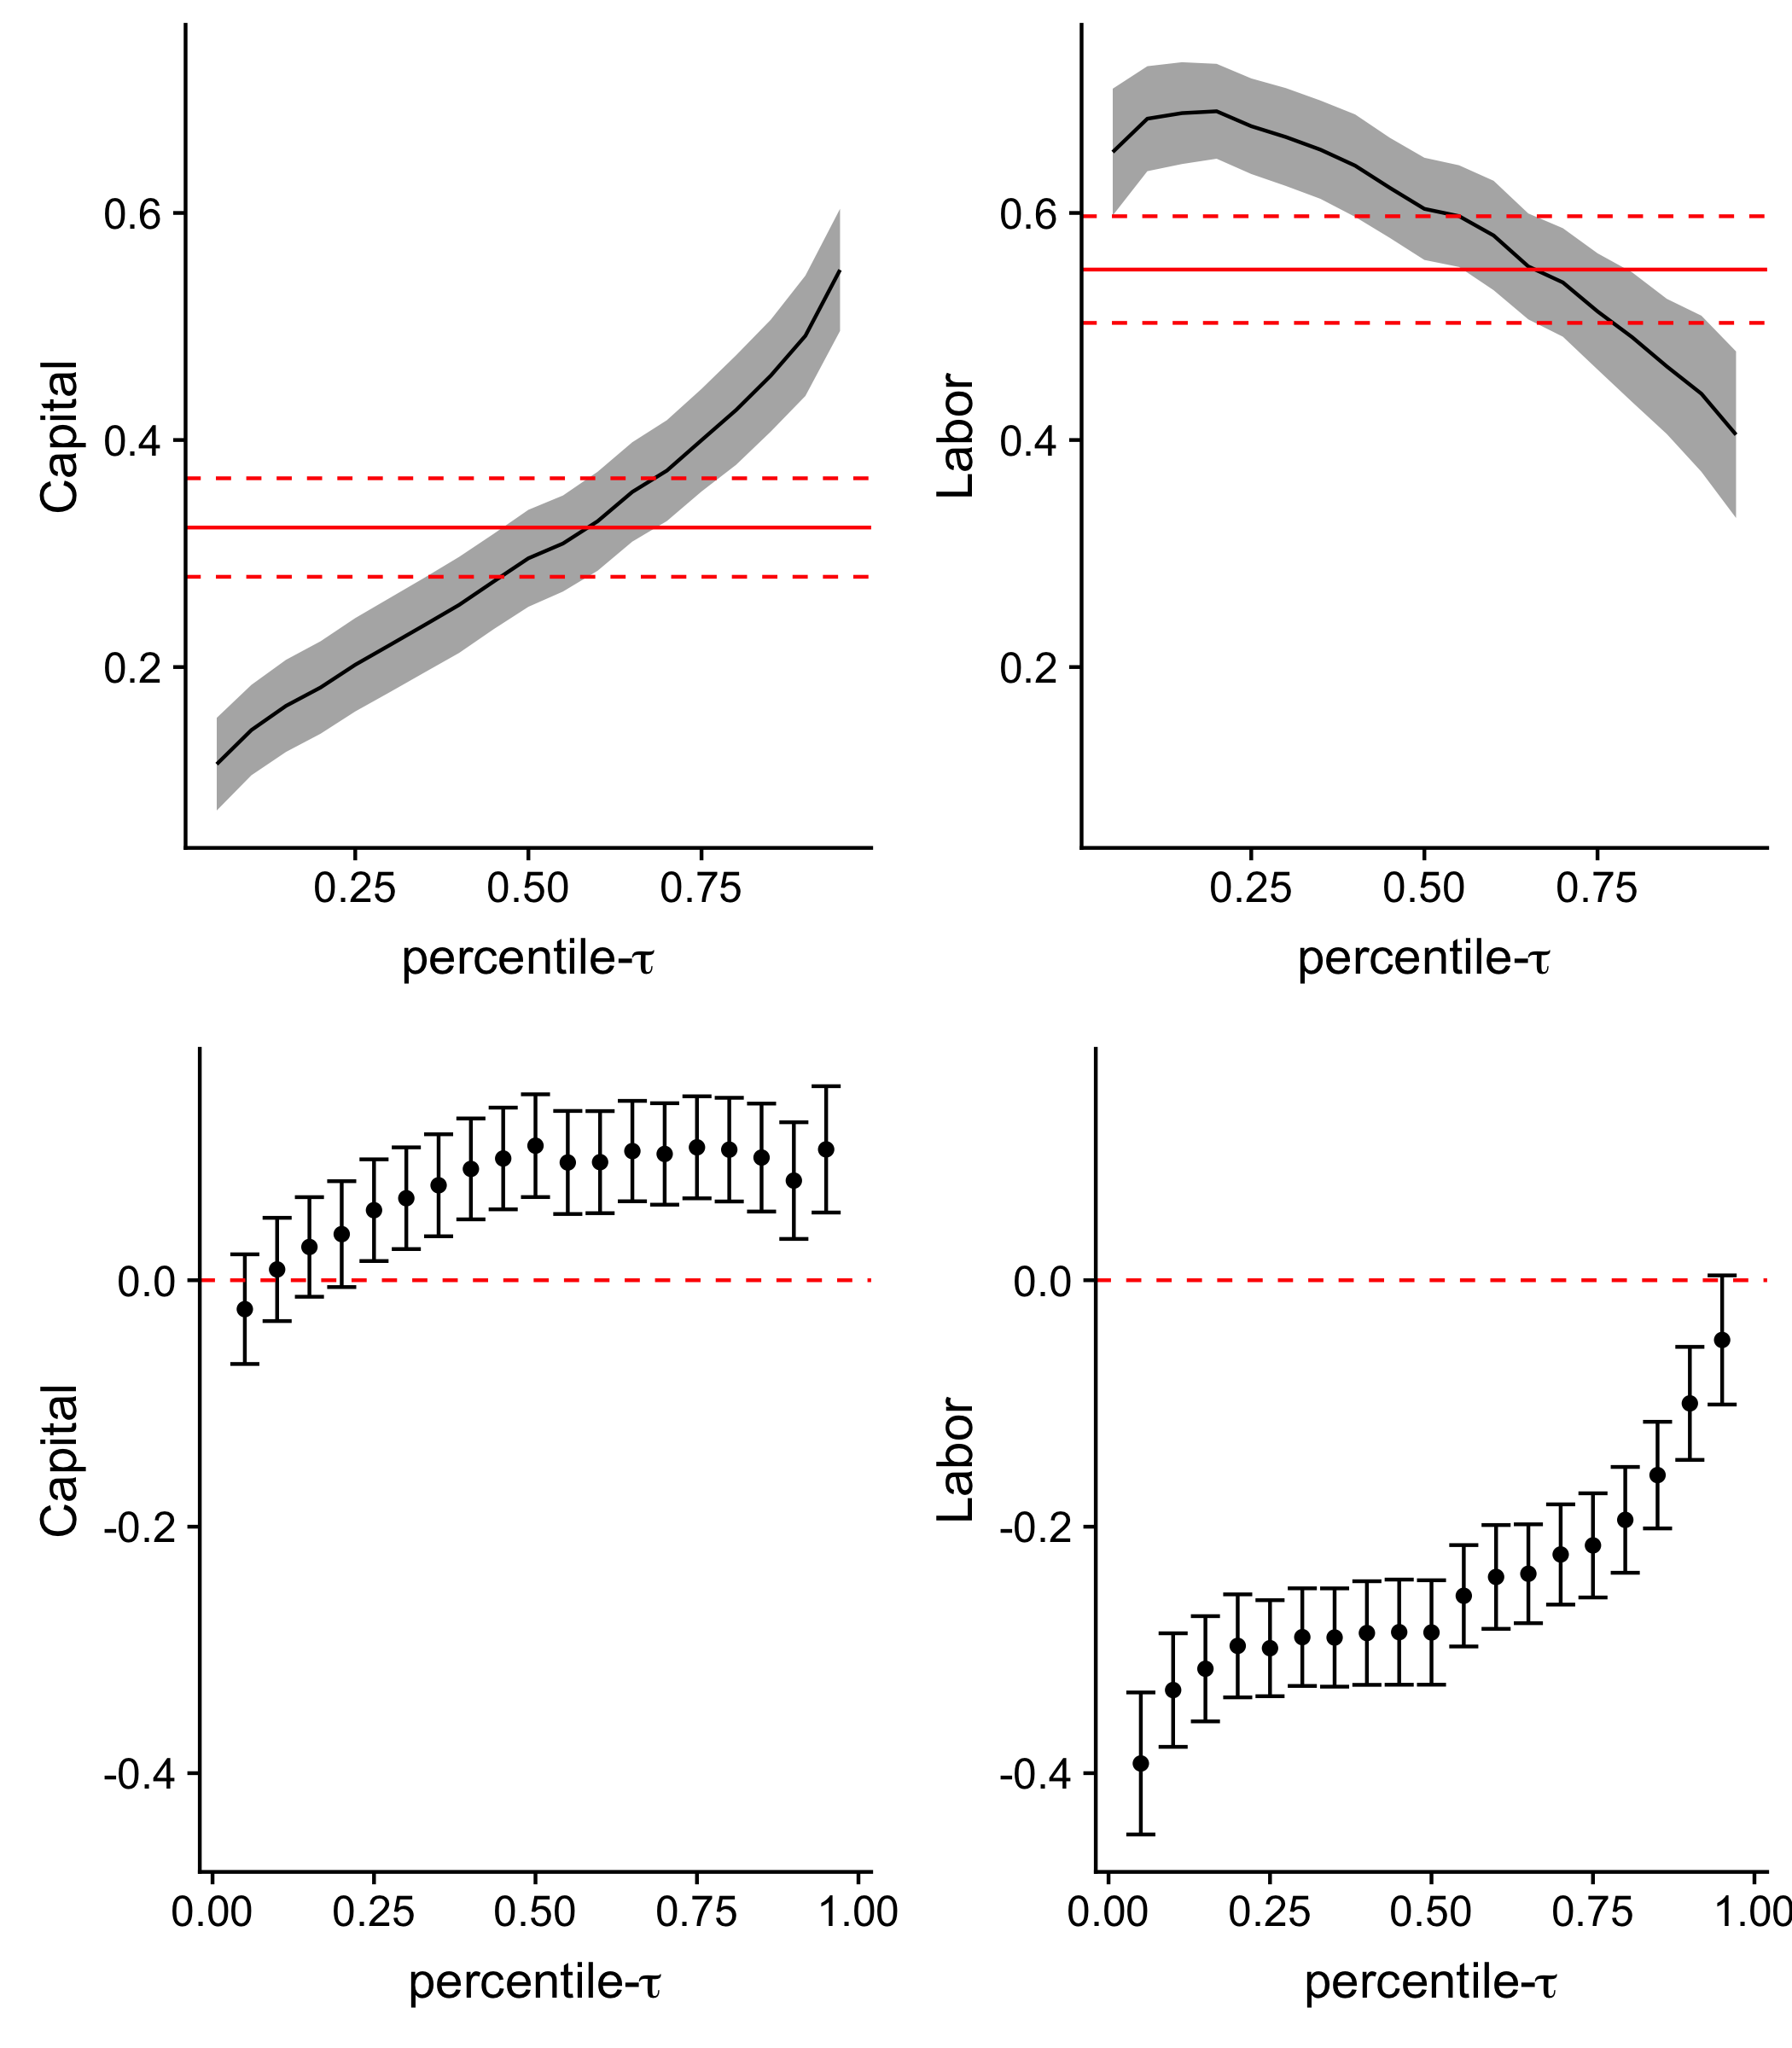
\includegraphics[width=9cm, height=9cm]{/Users/justindoty/Documents/Research/Dissertation/Production_QR_Proxy/Code/Empirical/Colombia/Plots/Coefficients/LP/QLP_Coef_Plot_ISIC_322.png}
\label{fig:LPCOL321}
\end{figure}

\begin{figure}[H]
\centering
\caption{Estimated Coefficients of Capital and Labor for Colombia: ISIC 381}
\includegraphics[width=9cm, height=9cm]{/Users/justindoty/Documents/Research/Dissertation/Production_QR_Proxy/Code/Empirical/Colombia/Plots/Coefficients/LP/QLP_Coef_Plot_ISIC_381.png}
\label{fig:LPCOL381}
\end{figure}

\begin{figure}[H]
\centering
\caption{Estimated Coefficients of Capital and Labor for all Colombian Manufacturing Plants}
\includegraphics[width=9cm, height=9cm]{/Users/justindoty/Documents/Research/Dissertation/Production_QR_Proxy/Code/Empirical/Colombia/Plots/Coefficients/LP/QLP_Coef_Plot_ISIC_All.png}
\label{fig:LPCOLall}
\end{figure}

\begin{figure}[H]
\centering
\caption{Mean and Median Estimates of Total Factor Productivity}
\includegraphics[width=12cm]{/Users/justindoty/Documents/Research/Dissertation/Production_QR_Proxy/Code/Empirical/Colombia/Plots/TFP/QLP_TFP_Plot.png}
\label{fig:LPTFPDens}
\end{figure}

\begin{figure}[H]
\centering
\caption{Chile Productivity Over Time}
\includegraphics[width=12cm]{/Users/justindoty/Documents/Research/Dissertation/Production_QR_Proxy/Code/Empirical/Colombia/Plots/TFP/QLP_TFPgrowth_Plot.png}
\label{fig:LPCHLpgrowth}
\end{figure}






















\end{document}